\documentclass{beamer}
\usepackage{caption}
\captionsetup[figure]{labelformat=empty}
\usepackage[utf8]{inputenc}
%Load useful packages
\usepackage{graphicx} % Allows including images
\usepackage{booktabs} % Allows the use of \toprule, \midrule and \bottomrule in tables
\usepackage{subcaption,color}
\usepackage[table]{xcolor}
\usepackage{multirow}

\usepackage{subfiles}
\usepackage{url}
\usepackage{amssymb}
\usepackage{multimedia}
\usepackage{bibentry}
\usepackage{algorithm,verbatim}
\usepackage{tikz,tikz-3dplot}
\usetikzlibrary{positioning,arrows,automata,external,hobby,decorations.pathreplacing,shapes,tikzmark}
\setbeamertemplate{navigation symbols}{}

\graphicspath{{../POPILS/}{../POPILS/images/}{../MPINNs_sorbonne/}{../../teaching/coursM2/figures/}{../../teaching/coursM2/MG/}}

\newcommand{\smallRe}{\hbox{\footnotesize I\hskip -2pt R}}
\newcommand{\calA}{{\cal A}} 
\newcommand{\calB}{{\cal B}} 
\newcommand{\calD}{{\cal D}} 
\newcommand{\calF}{{\cal F}} 
\newcommand{\tim}[1]{\;\; \text{#1} \;\;}
\newcommand{\ms}{\;\;\;\;}
\newcommand{\opA}{{\mathrm{A}}}
\newcommand{\opD}{\mathrm{L}}
\newcommand{\D}{\mathrm{L}}
\usepackage{leftidx}
\newcommand{\Raw}{\rightarrow}
\usepackage{appendixnumberbeamer}

%%%%% ML
\newcommand{\fsl}{f^{S_k^\ell}}
\newcommand{\fine}{\phi}
%\newcommand{\coarse}{\phi^H}
\newcommand{\coarse}{\phi}
\newcommand{\gk}{g_k}

\usepackage{tikz}
\usetikzlibrary{shapes.arrows}
\tikzset{
    myarrow/.style={
        draw,
        fill=orange,
        single arrow,
        minimum height=3.5ex,
        single arrow head extend=1ex
    }
}
\newcommand{\arrowright}{%
\tikz [baseline=-0.5ex]{\node [myarrow,rotate=-45] {};}
}
\newcommand{\arrowleft}{%
\tikz [baseline=-0.5ex]{\node [myarrow,rotate=-135] {};}
}


%\usepackage{algorithm}
\usepackage{algpseudocode,graphicx}
\newcommand\Fontvi{\fontsize{9}{9}\selectfont}
\newcommand\Fontvii{\fontsize{7}{7}\selectfont}
\newcommand\Fontviii{\fontsize{5}{5}\selectfont}
%Information to be included in the title page:
\title{Multilevel Physics Informed Neural Networks (MPINNs)}
\author{\underline{Elisa Riccietti}\\[3mm]
%\vspace{1cm}
Joint work with: S. Gratton - V. Mercier (IRIT), P. Toint (UNamur)}
\institute{LIP - ENS Lyon}
%\author{Valentin Mercier, \underline{Elisa Riccietti}, Serge Gratton, Philippe Toint}
%\institute{IRIT / \underline{ENS Lyon} / UNamur}


\date{\today}
%Logo in every slide

%%setting up some useful slide creation commands
%split slide
\newenvironment{splitframe}[5]
%[1] ==> 1 parameter passed through {}
%[2] ==> 2 parameters passed through {}{}
%[4] ==> 4 parameters passed through {}{}{}{}
    {
    \begin{frame}{#3}
    \begin{columns}
    \column{#1\linewidth}
    \centering
    #4
    \column{#2\linewidth}
    \centering
    #5
    \end{columns}
    \centering
    \vspace{\baselineskip} % adds one line space
    }
    %Inside the first pair of braces (ABOVE) is set what your new environment will do before the text within, then inside the second pair of braces (BELOW) declare what your new environment will do after the text. Note second pair can be empty braces too.
    {
    \end{frame}
    }
\AtBeginSection[]
{
    \begin{frame}
        \frametitle{Outline}
        \tableofcontents[currentsection]
    \end{frame}
}

\makeatletter
\renewcommand{\ALG@beginalgorithmic}{\small}
\makeatother



\begin{document}
%\setbeamertemplate{footline}[page number]
\addtobeamertemplate{navigation symbols}{}{%
    \usebeamerfont{footline}%
    \usebeamercolor[fg]{footline}%
    \hspace{1em}%
    \insertframenumber/\inserttotalframenumber
}
\begin{frame}
  \begin{center}
    \textbf{\LARGE  \alert{A multilevel stochastic  method with application to finite sum minimization}}
    \vspace{0.5cm}
      \end{center}
    \begin{columns}
    \begin{column}{0.6\textwidth}
    \textbf{ \alert{}}

    \vspace{0.5cm}
    \textbf{\underline{Elisa Riccietti} - LIP-ENS Lyon
    %and\\
   % Théo Mary
   }
   
   
    \vspace{0.5cm}
      \textbf{Filippo Marini - UNIBO}
      
     \vspace{0.2cm}
      \textbf{Margherita Porcelli - UNIFI}

     \vspace{1cm}
      SIOPT 2026 - Edinburgh 
      \includegraphics[scale=0.2]{../../loghi_firme/logo.png}
     \end{column}
    \begin{column}{0.4\textwidth}
  %  \includegraphics[width=0.8\textwidth]{images/grids.png}
     \centering
 \includegraphics[width=0.5\textwidth]{unc_sol.eps}    
 \includegraphics[width=0.5\textwidth]{sol_2.eps}    
\includegraphics[width=0.5\textwidth]{sol_1.eps}    


    \vfill
   

       \end{column}
            \end{columns}
             \end{frame}
  
  \begin{frame}{The concept}
  

{\bf AIM?} Given a large scale optimization problem, reduce the computational cost of the solution process \\
{\bf HOW? } Exploit the \alert{structure} to work at multiple resolutions
\vspace{0.3cm}

\begin{figure}\footnote{\tiny{Images taken from Introduction to Numerical Geodynamic Modelling  and \url{https://iipimage.sourceforge.io/documentation/images
}}}

\centering
\includegraphics[scale=0.3]{images/grids.png}
\hspace{1cm}
\includegraphics[scale=0.3]{images/pyramid.png}
\end{figure}
\begin{center}
\pause
{\color{red} \bf Multilevel methods (ML)}
\end{center}

  \end{frame}
  
  \begin{frame}{Outline}
  \begin{itemize}
  \item Part I: Origins of multilevel methods: multigrid
  \item Part II: Multilevel methods for nonlinear optimization
  \item Part III: Multilevel stochastic methods 
  \end{itemize}
  \end{frame}



\part{Origins of multilevel methods: multigrid}
\frame[plain]{\partpage}

\begin{frame}{Numerical solution of linear PDEs}







\begin{minipage}[t]{0.48\linewidth}
Given $f :\Omega\subset\mathbb{R}^d\rightarrow\mathbb{R}$, $g :\partial\Omega\rightarrow\mathbb{R}$ and a linear differential operator $D$, find $u:\mathbb{R}^d\rightarrow \mathbb{R}$ that solves
\begin{align*}
D(u(x))=f(x) \text{ in  } \Omega\\
u(x)=g(x) \text{ in  } \partial\Omega
\end{align*}
\centering
$$
\downarrow 
$$
Discretization
$$
\downarrow 
$$

Linear system 
$$
Au=f
$$

\end{minipage}\hfill
\begin{minipage}[t]{0.48\linewidth}

\begin{figure}
    \centering
    \includegraphics[width=0.8\linewidth]{images/grid2.png}
    \caption{Example: d=2, $\Omega=[0,1]\times[0,1]$
}
\end{figure}
 The size of the grid impacts:
 \begin{itemize}
 \item  the \alert{size} of the discrete problem
 \item the  \alert{accuracy} of the solution approximation
 \end{itemize}

\end{minipage}
\end{frame}











 












\begin{comment}
\begin{frame}{Multigrid methods}

{\bf Aim:} accelerate fixed point methods by exploiting multiple grids  \begin{columns}
\begin{column}{0.5\textwidth}
    \begin{figure}
    \centering
    
\includegraphics[width=0.90\linewidth]{images/MG.png}
\end{figure}
\end{column}
\begin{column}{0.40\textwidth}
    \begin{itemize}
\item \underline{Fine scales}: eliminate {\color{red}high frequency} components of the error
\item \underline{Coarse scales}: eliminate {\color{red}low frequency} components of the error
\end{itemize}
\end{column}
\end{columns}


\end{frame}
\end{comment}

\begin{frame}{Multigrid methods}

{\bf Aim:} accelerate fixed point methods by exploiting multiple grids  
\begin{minipage}[t]{0.48\linewidth}

    \vspace{1.5cm}

\begin{itemize}
    \item Fine grid: $A^hu^h=f^h$
    \vspace{3.5cm}
    \item Coarse grid: $A^{H}u^{H}=f^{H}$
    

\end{itemize} 

\end{minipage}
\begin{minipage}[t]{0.48\linewidth}
\begin{figure}
    \centering
    \includegraphics[width=0.8\linewidth]{images/grid2.png}
\end{figure}
\hspace{1.5cm}$\alert{R} \Downarrow$\hspace{1cm}$\alert{P} \Uparrow$

\begin{figure}
    \centering
    \includegraphics[width=0.8\linewidth]{images/grid0.png}
\end{figure}
\end{minipage}

    
   % When $A_h=A_H$ the residual equation simplifies:
    %$$
    %A_H(v_H+e_H^N)=R f_h
    %$$

\end{frame}



\begin{comment}
\begin{frame}{Multigrid ingredients}
\begin{enumerate}
\item Transfer operators
\begin{columns}
\begin{column}{0.5\textwidth}
Prolongation
\vspace{1cm}
%Build operators to transfer the information between the two levels
\begin{minipage}[t]{\linewidth}

 Interpolation

\begin{align*}
v_{2j}^h&=v_j^{2h}\\
v_{2j+1}^h&=\frac{1}{2}(v_j^{2h}+v_{j+1}^{2h})
\end{align*}
\begin{figure}
    \centering
    \includegraphics[width=0.7\linewidth]{images/P.png}
\end{figure}



\end{minipage}
\end{column}
\begin{column}{0.5\textwidth}
Restriction

%Build operators to transfer the information between the two levels
\begin{minipage}[t]{\linewidth}
\begin{itemize}
\item Injection:
$$
v_j^{2h}=v_{2j}^h
$$
\item Full weighting
$$
v_j^{2h}=\frac{1}{4} (v_{2j-1}^h+2v_{2j}^h+v_{2j+1}^h)
$$
\begin{figure}
    \centering
    \includegraphics[width=0.7\linewidth]{images/R.png}
\end{figure}
\end{itemize}

\end{minipage}

\end{column}
\end{columns}


\item $A^H$: discretization of differential operator on the coarse grid or 
\alert{Galerkin approximation}:
$$
A^{2h}=I_{h}^{2h}A^hI_{2h}^h
$$
\end{enumerate}
    
   % When $A_h=A_H$ the residual equation simplifies:
    %$$
    %A_H(v_H+e_H^N)=R f_h
    %$$

\end{frame}
\end{comment}

\begin{comment}
\begin{frame}{How to define the coarse level operator $A^{2h}$?}
Let  $v^h$  be a computed approximation to the exact solution $u^h$. 
Let  $e^h = u^h - v^h$ and assume that it lies entirely
in the range of interpolation: it exists  $u^{2h}\in\Omega^{2h}$ such that $e^h = I_{2h}^h u^{2h}$. The residual equation becomes:
$$
A^he^h=A^hI_{2h}^hu^{2h}=r^h
$$
We can see that
$A^hI_{2h}^hu^{2h}$ is zero at the odd points of $\Omega^h$, we can obtain $A^{2h}$ by dropping the odd rows, and we can do this by applying the restriction operator to both sides:
$$
I_{h}^{2h}A^hI_{2h}^h u^{2h}=I_{h}^{2h}r^h
$$
A plausible definition is thus 
$$
A^{2h}=I_{h}^{2h}A^hI_{2h}^h,
$$
the \alert{Galerkin condition}.
%We would get the same result if the original problem were simply discretized on Ω2h using the usual second-order finite differences. Therefore, by this definition, A2h really is the Ω2h version of Ah.
%The preceding argument was based on the assumption that the error eh lies entirely in the range of interpolation. This is not the case in general. If it were, then solving the Ω2h residual equation exactly and doing the two-grid correction would give the exact solution. Nevertheless, the argument does give a sensible def- inition for A2h. It also leads us to two important properties called the variational
\end{frame}
\end{comment}










\begin{frame}{General multigrid methods - V-cycle}

   % \includegraphics[width=\textwidth]{images/cycleV.png}
    % \includegraphics[scale=0.7]{images/v-cycle.png}
    \begin{columns}
     \begin{column}{0.4\textwidth}


              \includegraphics[width=\textwidth]{images/grids.jpeg}
                            \end{column}

        \begin{column}{0.6\textwidth}

              \includegraphics[width=\textwidth]{conv_MG}
              \end{column}
              
              \end{columns}

\centering
\tiny{Images taken from \url{https://en.wikipedia.org/wiki/Multigrid_method}}

\end{frame}


\part{From linear to nonlinear: multilevel optimization methods}
\frame[plain]{\partpage}


\begin{frame}{From linear to nonlinear: multilevel methods}
Multigrid methods work for linear systems: \alert{$Ax=b$}

%An extension exists for nonlinear equations: \alert{$\mathcal{A}(x)=b$} FAS (Full Approximation Scheme)

\begin{columns}
\begin{column}{0.5\textwidth}
But what happens if we want to tackle a more general \alert{optimization problem} with a hierarchical structure ? 
	\begin{equation*}
	\alert{\min_x f(x)}
	\end{equation*}
\end{column}
\begin{column}{0.5\textwidth}
\begin{figure}
\includegraphics[width=0.8\textwidth]{images/pyramid.png}
\end{figure}

\end{column}
\end{columns}


\end{frame}




\begin{frame}{Classical iterative optimization methods}
	
	 
	%Classical \alert{iterative} optimization methods:
	\begin{itemize}
	\item Build a \alert{model} ($B_k\sim \nabla^2 f(x_k)$ or $B_k=0$):
	\begin{equation*}
	f(x_k+s)\simeq T_{k}(s)=f(x_k)+s^T\nabla f(x_k)+\frac{1}{2}s^TB_ks
	\end{equation*}
	%with $T_{k}(x_k,s)$ Taylor model, .\\
	\vspace{-0.5cm}
	\pause
	\item Compute a \alert{step} $s_k$ ($r(\lambda_k)$ regularization term):
	\begin{equation*}
	\underbrace{\min_s m_{k}(s)=T_{k}(s)+r(\lambda_k)}_{\text{bottleneck: subproblem solution}},\qquad \lambda_k>0
	\end{equation*}
	\vspace{-0.5cm}

	\end{itemize}






	
		\vspace{0.5cm}


\begin{block}{ {\bf Possible solution}:  \alert{multilevel methods} }
		
		\begin{small}
	\begin{thebibliography}{9}
		\setbeamertemplate{bibliography item}[article]
		\bibitem{D} \alert{MG/OPT: } \textit{A multigrid approach to discretized optimization problems}, {\color{black} Nash}, {\color{black} 2000}
		\bibitem{C} \alert{RMTR: } \textit{Recursive trust-region methods}, {\color{black} S. Gratton, A. Sartenaer and  Ph. L. Toint, 2008}
		%\bibitem{E} \textit{On high-order multilevel optimization strategies}, {\color{black} H. Calandra, S. Gratton, E. Riccietti, X. Vasseur}, {\color{black} 2020}

	\end{thebibliography} 
	\end{small}


	\end{block}		
\end{frame}



	
	
	
			
	\begin{frame}\frametitle{Hierarchy of problems {\small ($n_{\ell_{\max}}> n_{\ell_{\max}-1} > \dots >n_0$)}}
{\footnotesize
 \begin{columns}
  \begin{column}{0.2\textwidth}
 \includegraphics[width=0.9\textwidth]{grid-14.mps}    
\end{column}
\begin{column}{0.6\textwidth}
      \begin{block}{} \centerline{$\smash{\mbox{Finest Level  $f^{\ell_{\max}} : \mathbb{R}^{n_{\ell_{\max}}}\to \mathbb{R}$ }}\vphantom{level}$} \end{block} 
{\color{blue}Restriction $\downarrow$ $R^{\ell_{\max}}$} \hfill  \alert{$P^{\ell_{\max}}$ $\uparrow$ Prolongation}  \end{column}
\begin{column}{0.2\textwidth}
\includegraphics[width=0.9\textwidth]{sol_6.eps}    
   \end{column}
     \end{columns} 
 \begin{columns}
  \begin{column}{0.2\textwidth}
 \includegraphics[width=0.9\textwidth]{grid-13.mps}    
\end{column}
\begin{column}{0.6\textwidth}
      \begin{block}{} \centerline{$\smash{\mbox{Fine Level  $f^{\ell_{\max}-1} : \mathbb{R}^{n_{\ell_{\max}-1}}\to \mathbb{R}$ }}\vphantom{level}$} \end{block}  
{\color{blue}Restriction $\downarrow$ $R^{\ell_{\max}-1}$} \hfill  \alert{$P^{\ell_{\max}-1}$ $\uparrow$ Prolongation} 
\end{column}
\begin{column}{0.2\textwidth}
 \includegraphics[width=0.9\textwidth]{unc_sol.eps}    
   \end{column}
     \end{columns} 

\begin{columns}
  \begin{column}{0.2\textwidth}
  \end{column}
\begin{column}{0.6\textwidth}
     \begin{block}{} \centerline{$\smash{\vdots}\vphantom{level}$} \end{block}  
{\color{blue}Restriction $\downarrow$ $R^{2}$}\hfill  \alert{$P^{2}$ $\uparrow$ Prolongation} 
  \end{column}
\begin{column}{0.2\textwidth}
   \end{column}
     \end{columns} 

 \begin{columns}
  \begin{column}{0.2\textwidth}
 \includegraphics[width=0.9\textwidth]{grid-12.mps}    
\end{column}
\begin{column}{0.6\textwidth}
      \begin{block}{} \centerline{$\smash{\mbox{Coarse Level  $f^2 : \mathbb{R}^{n_2}\to \mathbb{R}$ }}\vphantom{level}$} \end{block} 
{\color{blue}Restriction $\downarrow$ $R^1$} \hfill  \alert{$P^{1}$ $\uparrow$ Prolongation}  \end{column}
\begin{column}{0.2\textwidth}
\includegraphics[width=0.9\textwidth]{sol_2.eps}    
   \end{column}
     \end{columns} 
 \begin{columns}
  \begin{column}{0.2\textwidth}
 \includegraphics[width=0.9\textwidth]{grid-11.mps}    
\end{column}
\begin{column}{0.6\textwidth}
      \begin{block}{} \centerline{$\smash{\mbox{Coarsest Level  $f^0 : \mathbb{R}^{n_0}\to \mathbb{R}$ }}\vphantom{level}$} \end{block} 
 \end{column}
\begin{column}{0.2\textwidth}
\includegraphics[width=0.9\textwidth]{sol_1.eps}    
   \end{column}
     \end{columns} 
}


\end{frame}


\begin{frame}{Example 1: image restoration}





\begin{columns}
\begin{column}{0.5\textwidth}
\hspace{1cm}
\centering
\includegraphics[scale=0.12]{images/vitt_vert}
\end{column}

\hspace{1cm}
\vspace{-10cm}
\begin{column}{0.5\textwidth}
\centering
\includegraphics[scale=0.2]{images/wavelets}
\end{column}
\end{columns}


\end{frame}

\begin{frame}{Example 2: hyperspectral imaging }
%\mbox{} \\
%\mbox{} \\
\centering
%\includegraphics[trim={1em 0.2em 1em 0.1em},clip,width = 1\textwidth]{images/TransfertInfoIHS.pdf}
    \includegraphics[width=0.9\textwidth]{TransfertInfoHYSpatial-crop.pdf}
        \includegraphics[width=1\textwidth]{TransfertInfoHYSpectral-crop.pdf}
\end{frame}


\begin{frame}{Example 3: neural networks }


\centering
\includegraphics[width=\textwidth]{nn_hierarchical}

\end{frame}

		
		
\begin{comment}
\begin{frame}{Classical one-level method}

Let $x_k$ be the current approximation. 

We look for $s_k$ to define the new approximation

\begin{center}
		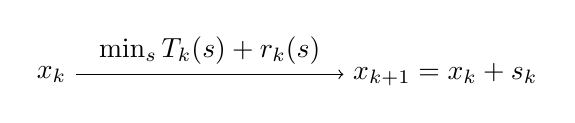
\begin{tikzpicture}[scale=2]
		\node(a) at (0,1){$x_k$};
		\pause
		 		\node(d) at (2.5,1){$x_{k+1} = x_k+s_k$};
		\draw (a) edge[->] node[above]{$\min_{s} T_k(s)+r_k(s)$} (d);
	\end{tikzpicture}
	\end{center}


\end{frame}
\begin{frame}{Multilevel strategy}
 % \vspace{-0.2cm}
	\begin{block}{Hierarchy of problems}
		\begin{itemize}
      \item $\{f^h(x^h)\}$, $x^h\in\mathbb{R}^{n_h}$
      \item \alert{$n_{H} < n_h$} $\Raw$ $f^{H}$ is cheaper to optimize compared with $f^h$
      \item $\mu^{H}$ model for $f^{H}$
		\end{itemize}
	\end{block}
	\end{frame}
	
	\begin{frame}{Multilevel strategy: step computation }
	
	Two choices:
	\begin{enumerate}
	\item \alert{Classical fine step}
	\item Coarse step
		\end{enumerate}
		
	\begin{center}
		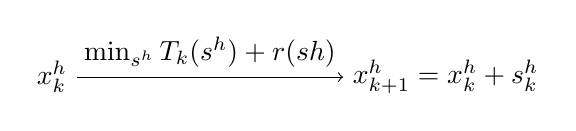
\begin{tikzpicture}[scale=2]
		\node(a) at (0,1){$x_k^h$};
		 		\node(d) at (2.5,1){$x_{k+1}^h = x_k^h+s_k^h$};

		\draw (a) edge[->] node[above]{$\min_{s^h} T_k(s^h)+r(sh)$} (d);

		 
		
		\end{tikzpicture}
	\end{center}
	

	
	
\end{frame}


\begin{frame}{Multilevel strategy}
 
	Two choices:
	\begin{enumerate}
	\item Classical fine step
	\item \alert{Coarse step}
		\end{enumerate}

	\begin{center}
		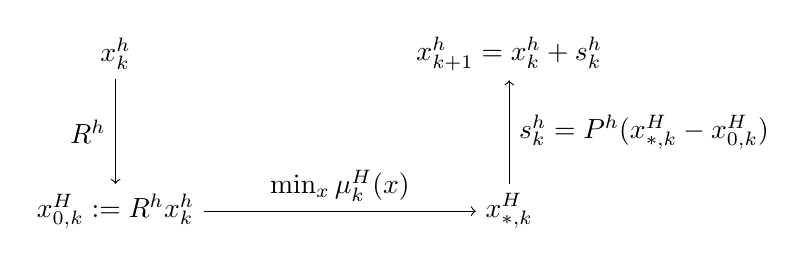
\begin{tikzpicture}[scale=2]
		\node(a) at (0,1){$x_k^h$};
		 
		\node(b) at (0,0){$x_{0,k}^{H} := R^h x_k^h$};
		\draw (a) edge[->] node[left]{$R^h$} (b);
		 
		\node(c) at (2.5,0){$x_{*,k}^{H}$};
		\draw (b) edge[->] node[above]{$\min_x \mu_k^{H}(x)$}(c);
		 
		\node(d) at (2.5,1){$x_{k+1}^h = x_k^h+s_k^h$};
		\draw (c) edge[->] node[right]{$s_k^h=P^h(\alert{x_{*,k}^{H}-x_{0,k}^{H}})$} (d);
		
		\end{tikzpicture}
	\end{center}
	

	
	
\end{frame}

\end{comment}


\begin{frame}{Classical one-level method}

		
	\includegraphics[width=\textwidth]{iter_fine}
\end{frame}

\begin{frame}{Multilevel strategy: step computation }
	
	Two choices:
	\begin{enumerate}
	\item Classical fine step
	\item Coarse step
		\end{enumerate}
		\vspace{1cm}
		\centering
\includegraphics[width=\textwidth]{scheme_iter}
		\end{frame}

		
		
		

		
		\begin{frame}{Coarse step }

		
	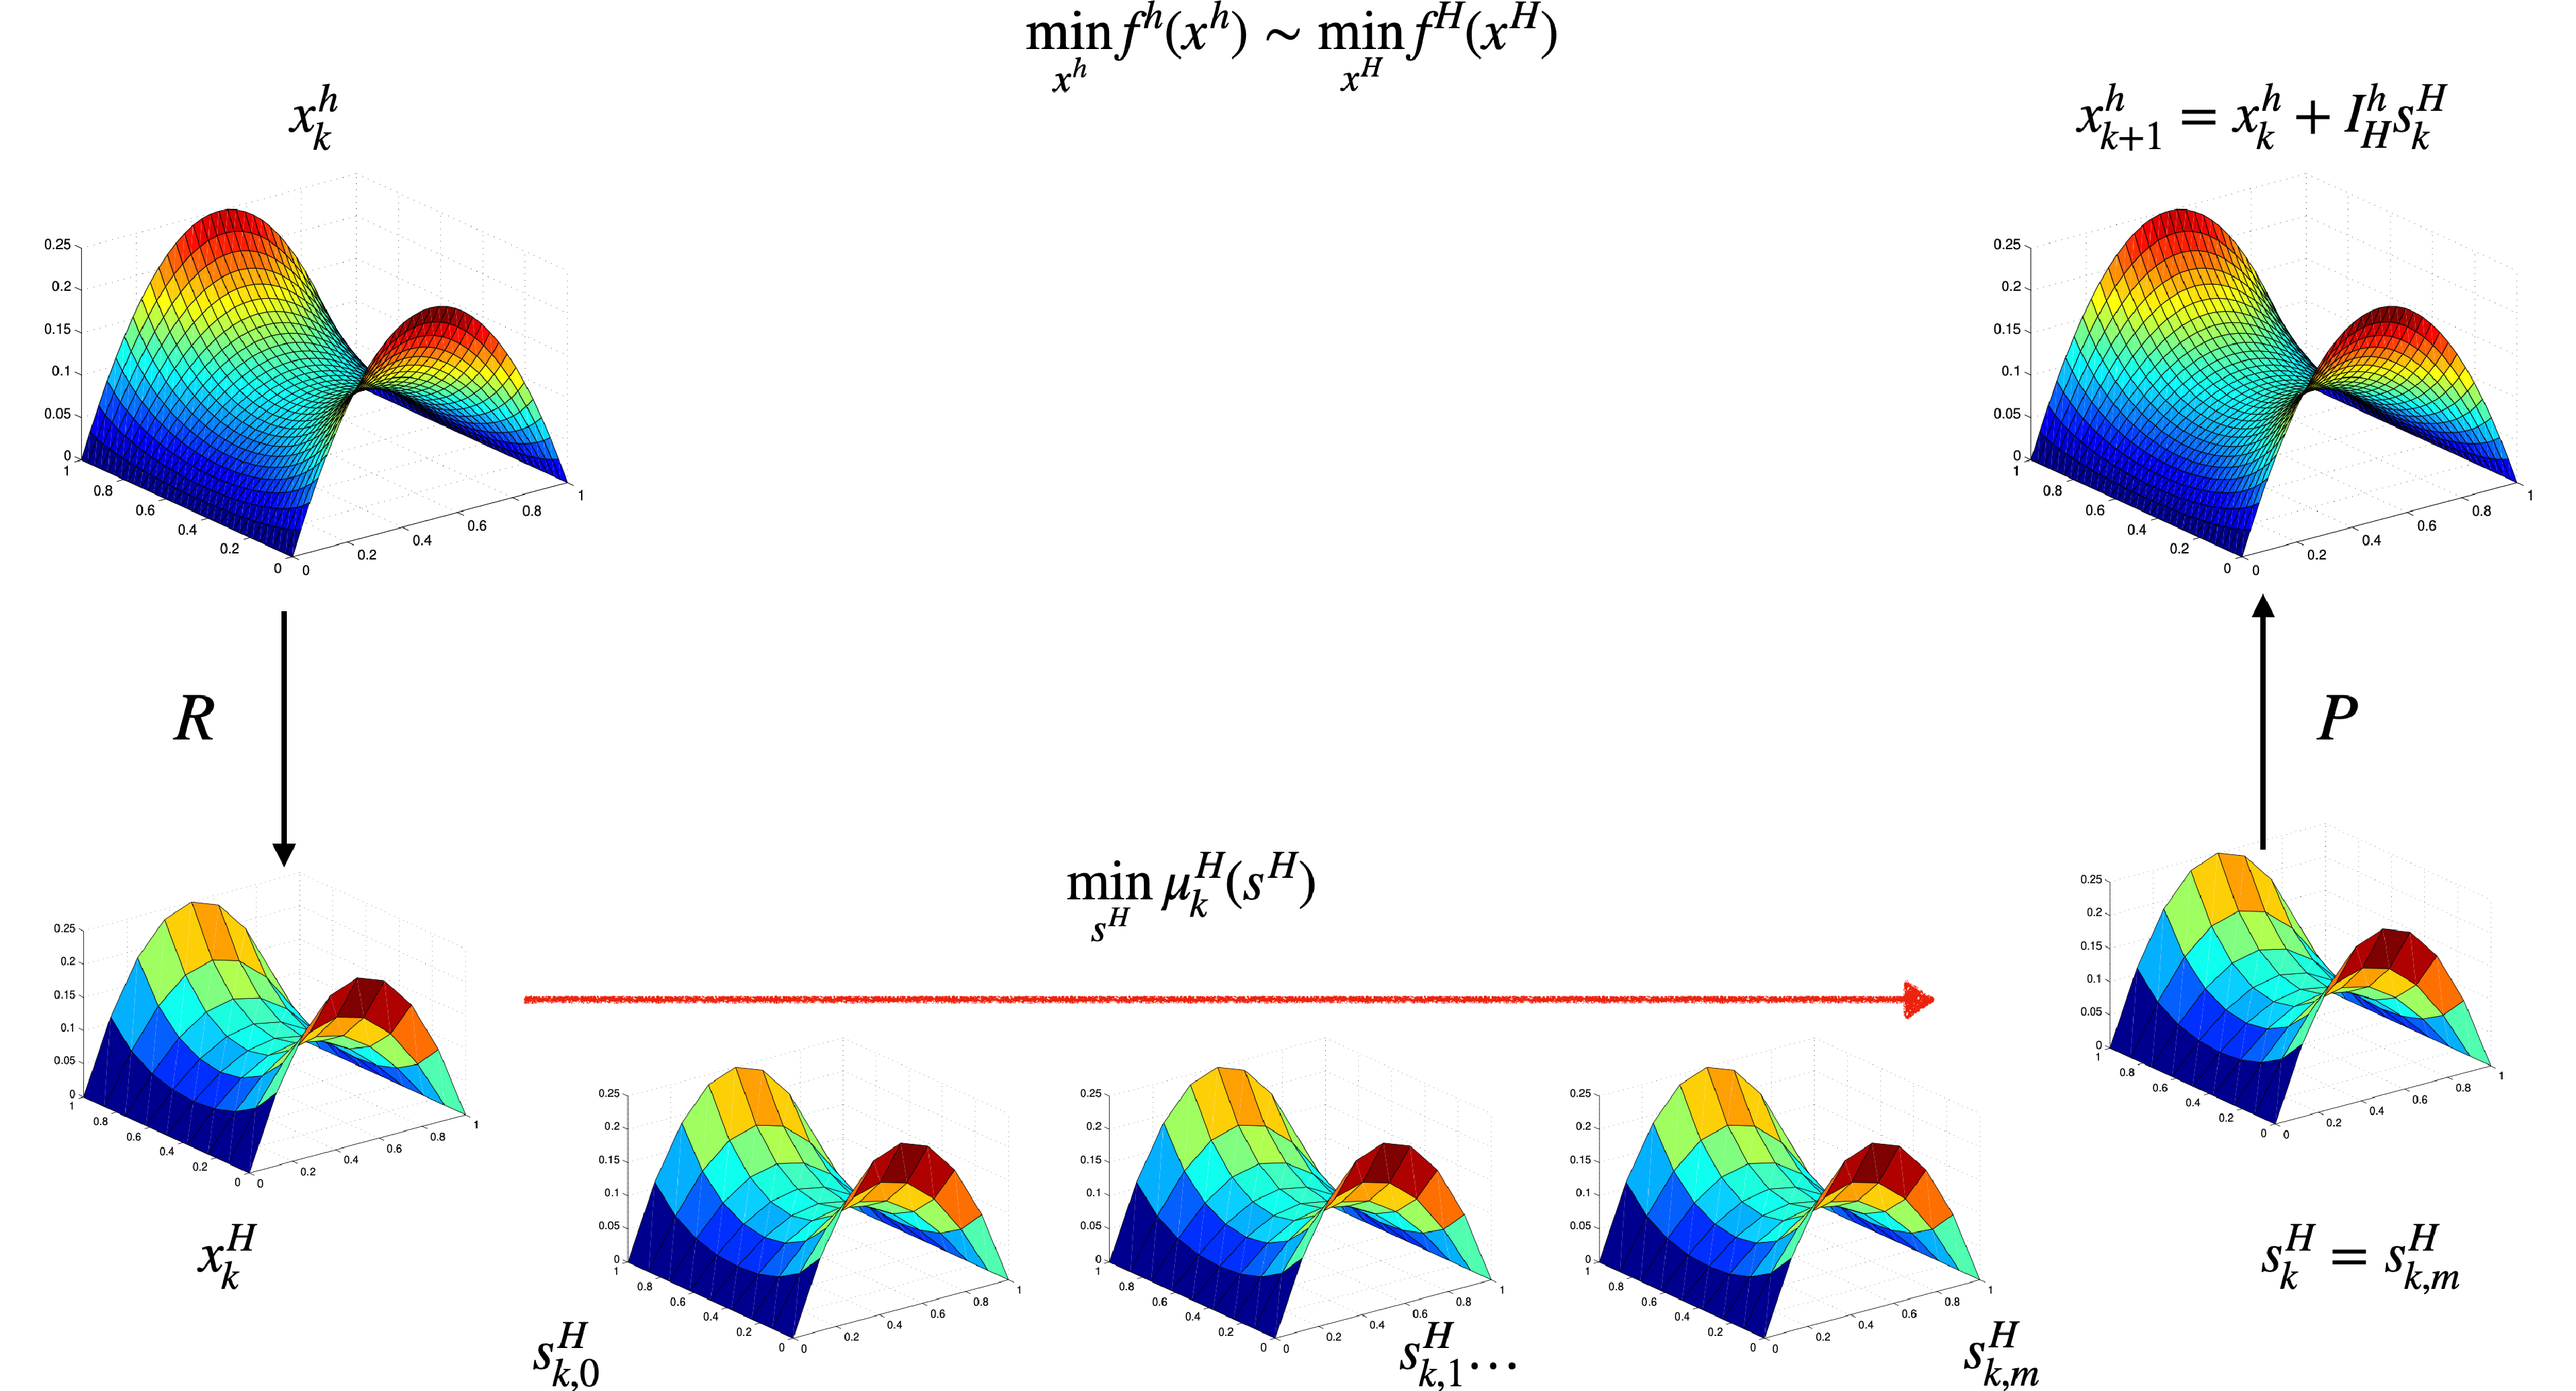
\includegraphics[width=\textwidth]{figures/iter_coarse2}
\end{frame}


%\begin{frame}{An iteration of a multilevel procedure - two-levels}
%\centering
%\includegraphics[height = 6cm]{images/kiter}
%\pause 
%\alert{$R,P$?} \hspace{5cm} \alert{$F_H$?}
%\end{frame}





		
	

\begin{frame}{Definition of lower level model: first order coherence}
    %\includesvg[width = 0.5\textwidth]{images/slide_first_order_coherence/First_order_coherence.svg}
    \centering
   % \includegraphics[width = 1\textwidth]{images/slide_first_order_coherence/figure-presentation_multiniveau_bonnesdimensions.pdf}
        \includegraphics[width = 1\textwidth]{../../projects/HDR/figures/correction.pdf}

   $v_k^{H}=R\nabla f^h(x_k^{h})-\nabla f^{H} (x_k^{H})\rightarrow \underbrace{\nabla \mu_{k}^{H}(0^{H})=R\nabla f^h(x_k^h)}_{\text{first-order coherence}}$
\end{frame}


			









	


%\end{comment}

\begin{frame}{Numerical results for 5 levels MG/OPT with line-search}

Problem: 

\centering
\includegraphics[width=0.5\textwidth]{pb_nash}
\includegraphics[width=0.6\textwidth]{run_nash}

\begin{small}
	\begin{thebibliography}{9}
		\setbeamertemplate{bibliography item}[article]
		\bibitem{D}  \textit{Using Inexact Gradients in a Multilevel Optimization Algorithm}, {\color{black} M. Lewis, S. G. Nash}, {\color{black} 2013}

	\end{thebibliography} 
	\end{small}








\end{frame}
	
\begin{frame}{A very active field}
\centering
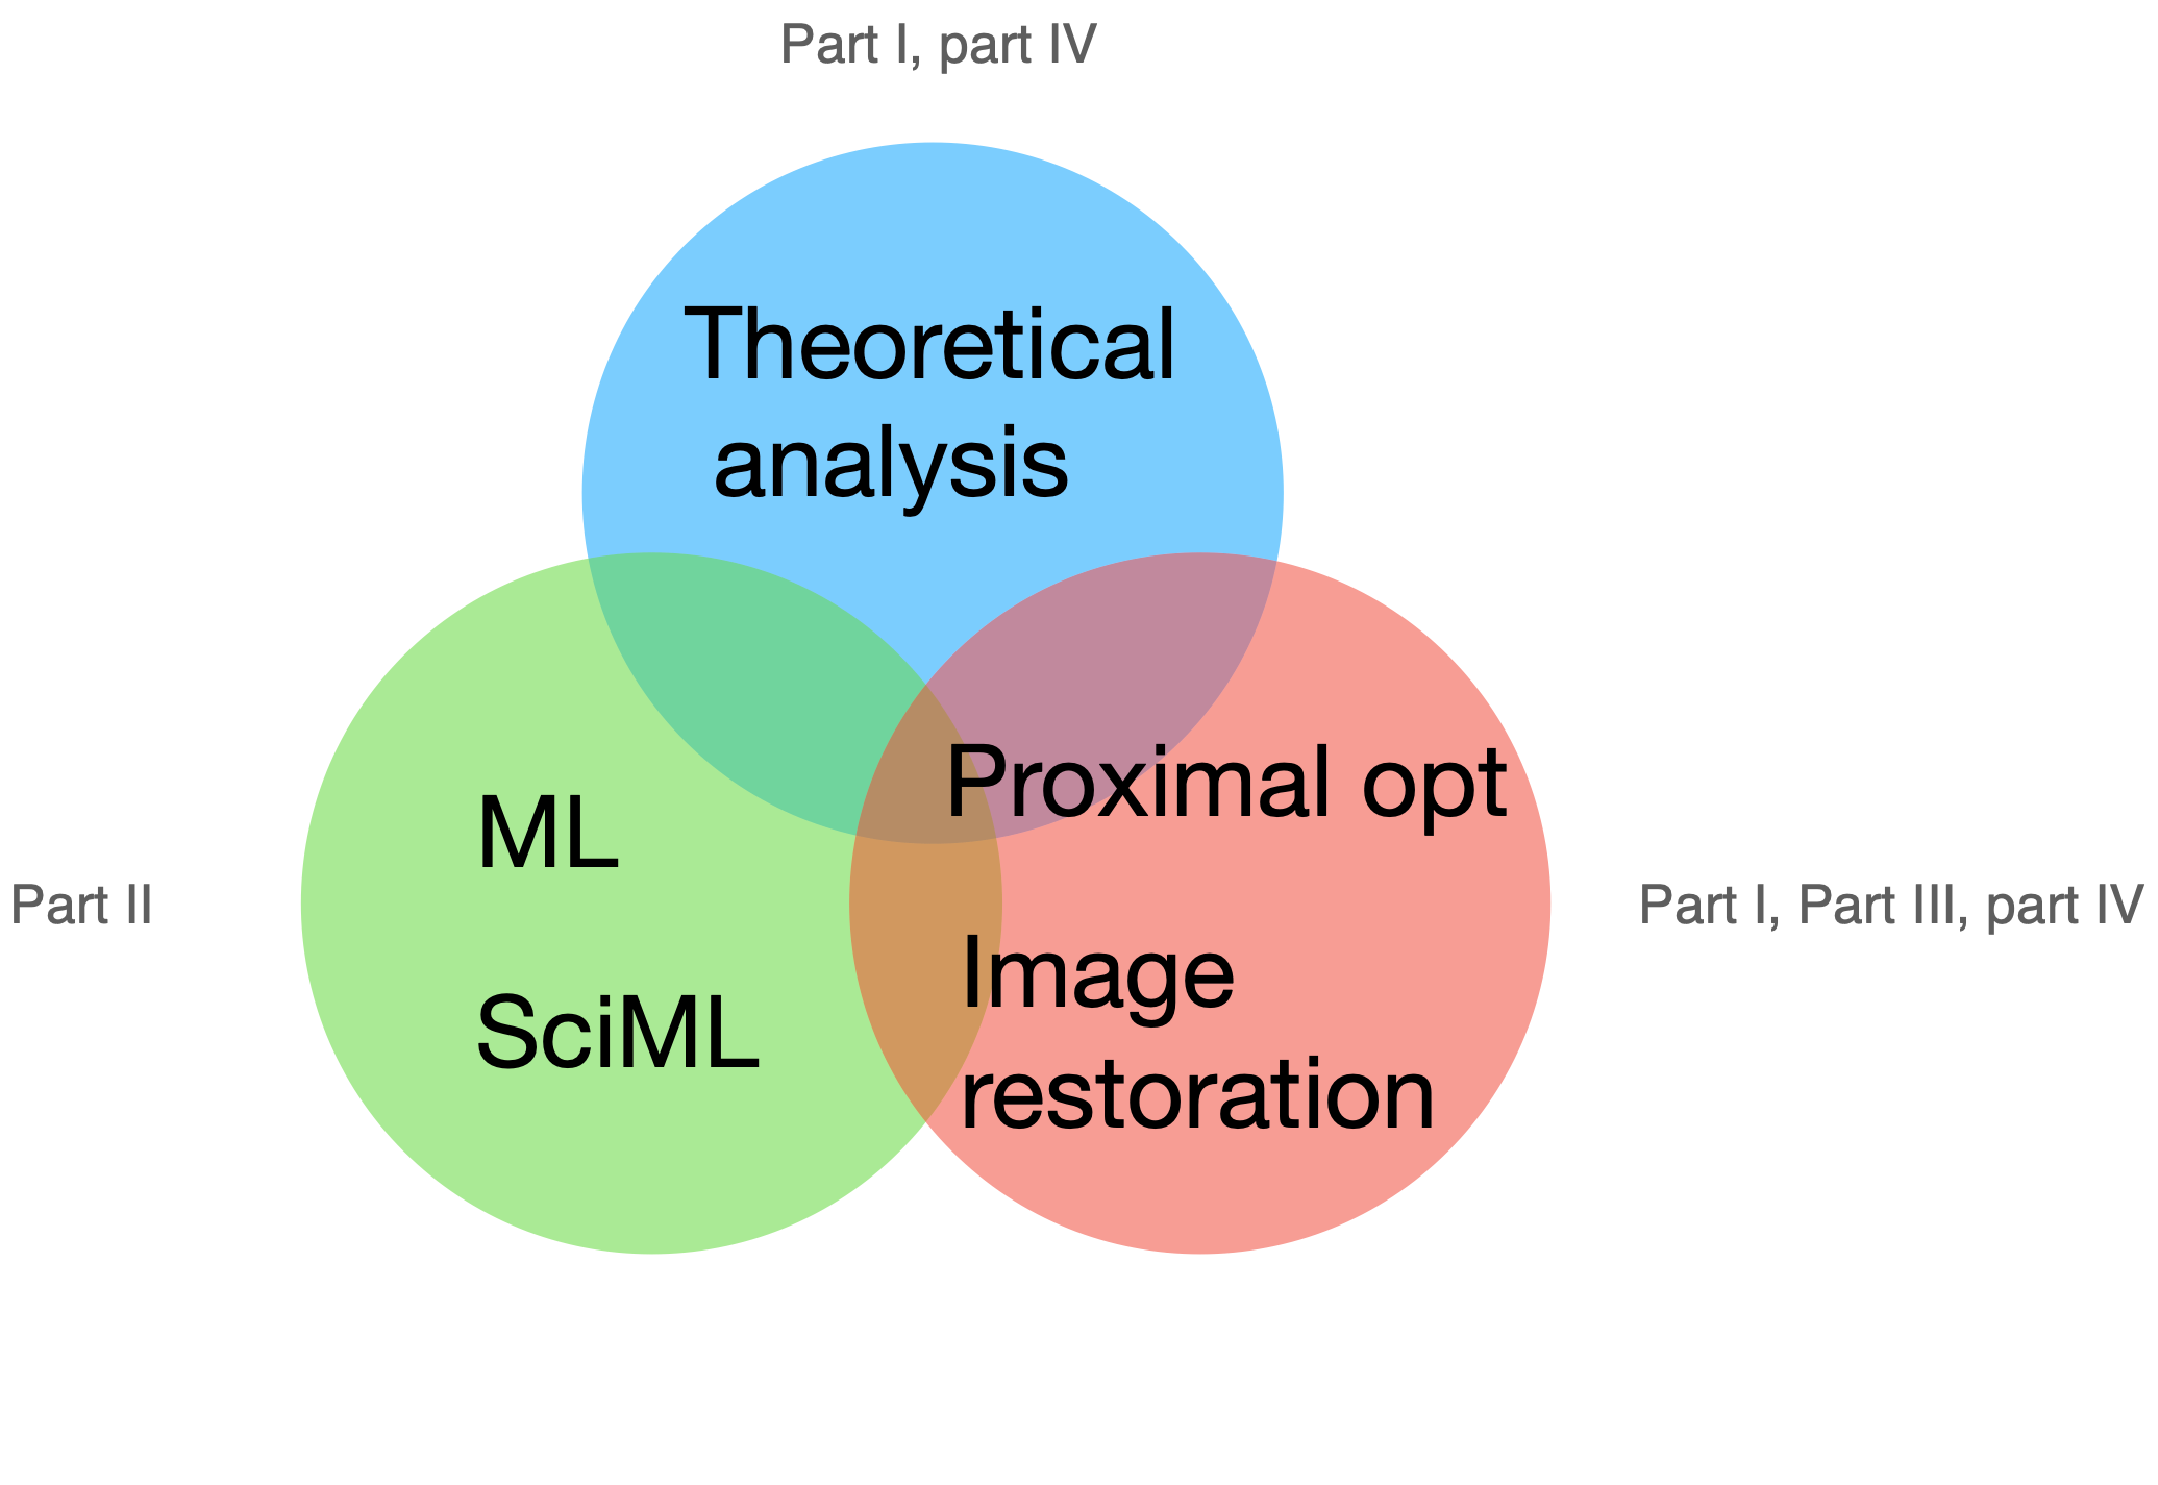
\includegraphics[scale=0.2]{figures/parts}
\end{frame}	


	\part{Stochastic multilevel optimization}
	\frame[plain]{\partpage}
	
	
	
	\begin{frame}{Stochastic optimization problems}
	What if my problem is stochastic? 
	$$
	\min_x f(x)
	$$
	where $f$ can only be computed \alert{with some noise}.
	
	
	
	\begin{block}{Example - \emph{Expected risk minimization problems} }
 Given a loss function $\mathcal{L}:\mathcal{Y}\times\mathcal{Y}\rightarrow\mathbb{R}$, a parametric model $m_x:\mathcal{Z}\rightarrow \mathcal{Y}$ and a probability distribution $P$ on $\mathcal{Z}\times\mathcal{Y}$
 \begin{equation*}
     \min_{x \in \mathbb{R}^n} \mathbb{E}_P[\mathcal{L}(y,m_x(z))]
\end{equation*}
 
 \end{block}
 
 \begin{block}{Example - \emph{Montecarlo simulations} }
Let $\xi$ be a random variable defined on the probability space $(\Omega,P)$. 
Let $f(x)=\mathbb{E}(F(x,\xi))$, with $F:\mathbb{R}^n\times \Omega\rightarrow \mathbb{R}$. 

%$F(x,\xi)$ can represent for instance the fit of the solution of a stochastic PDE to some data. $F$ can be approximated at fine level by the stochastic  approximations 
%$F_{h_k}(x,\xi)$, the output of a PDE solver with mesh size $h_k>0$ and  
%$f$ can then be approximated by the Montecarlo estimator 
%$$
%\hat{f}_{N_k,h_k}(x)=\frac{1}{N_k} \sum_{i=1}^{N_k} F_{h_k}(x,\xi_i)
%$$
  % where $\xi_1,\dots,\xi_{N_k}$ are iid samples drawn from $P$. 
   %The coarse approximations can be built either: 
  % \begin{enumerate}
     %  \item \emph{In the function space}, by defining 
      % $$
%\phi^{\ell}_k(x)=\frac{1}{N_k^\ell} \sum_{i=1}^{N_k^\ell} F_{h^\ell_k}(x,\xi_i)
%$$
 %   with $h_k^\ell\geq h_k^{\ell+1}\geq h_k$ and/or $N_k^{\ell}\leq N_k^{\ell+1}\leq N_k$ for al $\ell$ and for all $k$.    
    %   \item \emph{In the variables space} by defining 
      % $$
%\phi^{\ell}_k(\bar{x})=\frac{1}{N_k} \sum_{i=1}^{N_k} F_{h_k}(\bar{x},\xi_i), \quad \bar{x}\in\mathbb{R}^{n_k^\ell}
%$$
%with $n^\ell_k\leq n_k^{\ell+1}\leq n$ for all $\ell$ and for all $k$.
  % \end{enumerate}
\end{block} 


 
 
 \end{frame}
 
 \begin{frame}{Limitation of existing methods}
 \underline{Stochastic methods}: 
 \begin{itemize}
 \item 
 Accuracy of the function approximations \alert{grows} asymptotically, which leads to iterations that are more and more expensive:
 $$
 \|f(x)-\tilde f(x)\|\leq \epsilon_k, \quad \epsilon_k\rightarrow 0
 $$
  \item Such methods control the accuracy of the function estimates but not the \alert{size of the variables}.   
 \end{itemize}
 \vspace{0.5cm}
 
%Challenge: develop \alert{scalable} stochastic methods, able to handle the increasing costs of large scale stochastic optimization problems. 

\underline{Multilevel framework}:
\begin{itemize}
 \item Limited to \alert{deterministic} contexts
 \item Still needs to handle \alert{full problem} at the finest scale
 \end{itemize}
 
 \pause
 \begin{center}
 $\rightarrow$ \alert{Stochastic multilevel methods!}
 \end{center}
 \end{frame}
 
 

 \begin{comment}
 \begin{frame}{Can we leverage the multilevel framework? }
\begin{itemize}
\item  \underline{Fine level}: increasingly accurate approximations to $f$
\vspace{0.5cm}
\item  \underline{Coarse levels}: cheaper approximations $\phi_k^\ell$
\end{itemize}
\begin{columns}

%---------------------------------
\begin{column}{0.5\textwidth}

\fbox{%
\begin{minipage}{\linewidth}
\centering

%\vspace{0.2cm}

$$
f:\boxed{\mathcal{X}}\rightarrow \mathcal{Y}
$$

Hierarchy in the variables space:

\begin{tiny}
${\color{green}\rm{dim}(\mathcal{V}^0)}
{\color{black}\leq\dots\leq}
{\color{orange}\rm{dim}(\mathcal{V}^\ell)}
{\color{black}\leq\dots\leq}
{\color{red}\rm{dim}(\mathcal{V}^{\ell_{\max}})}$
\end{tiny}

\vspace{0.3cm}

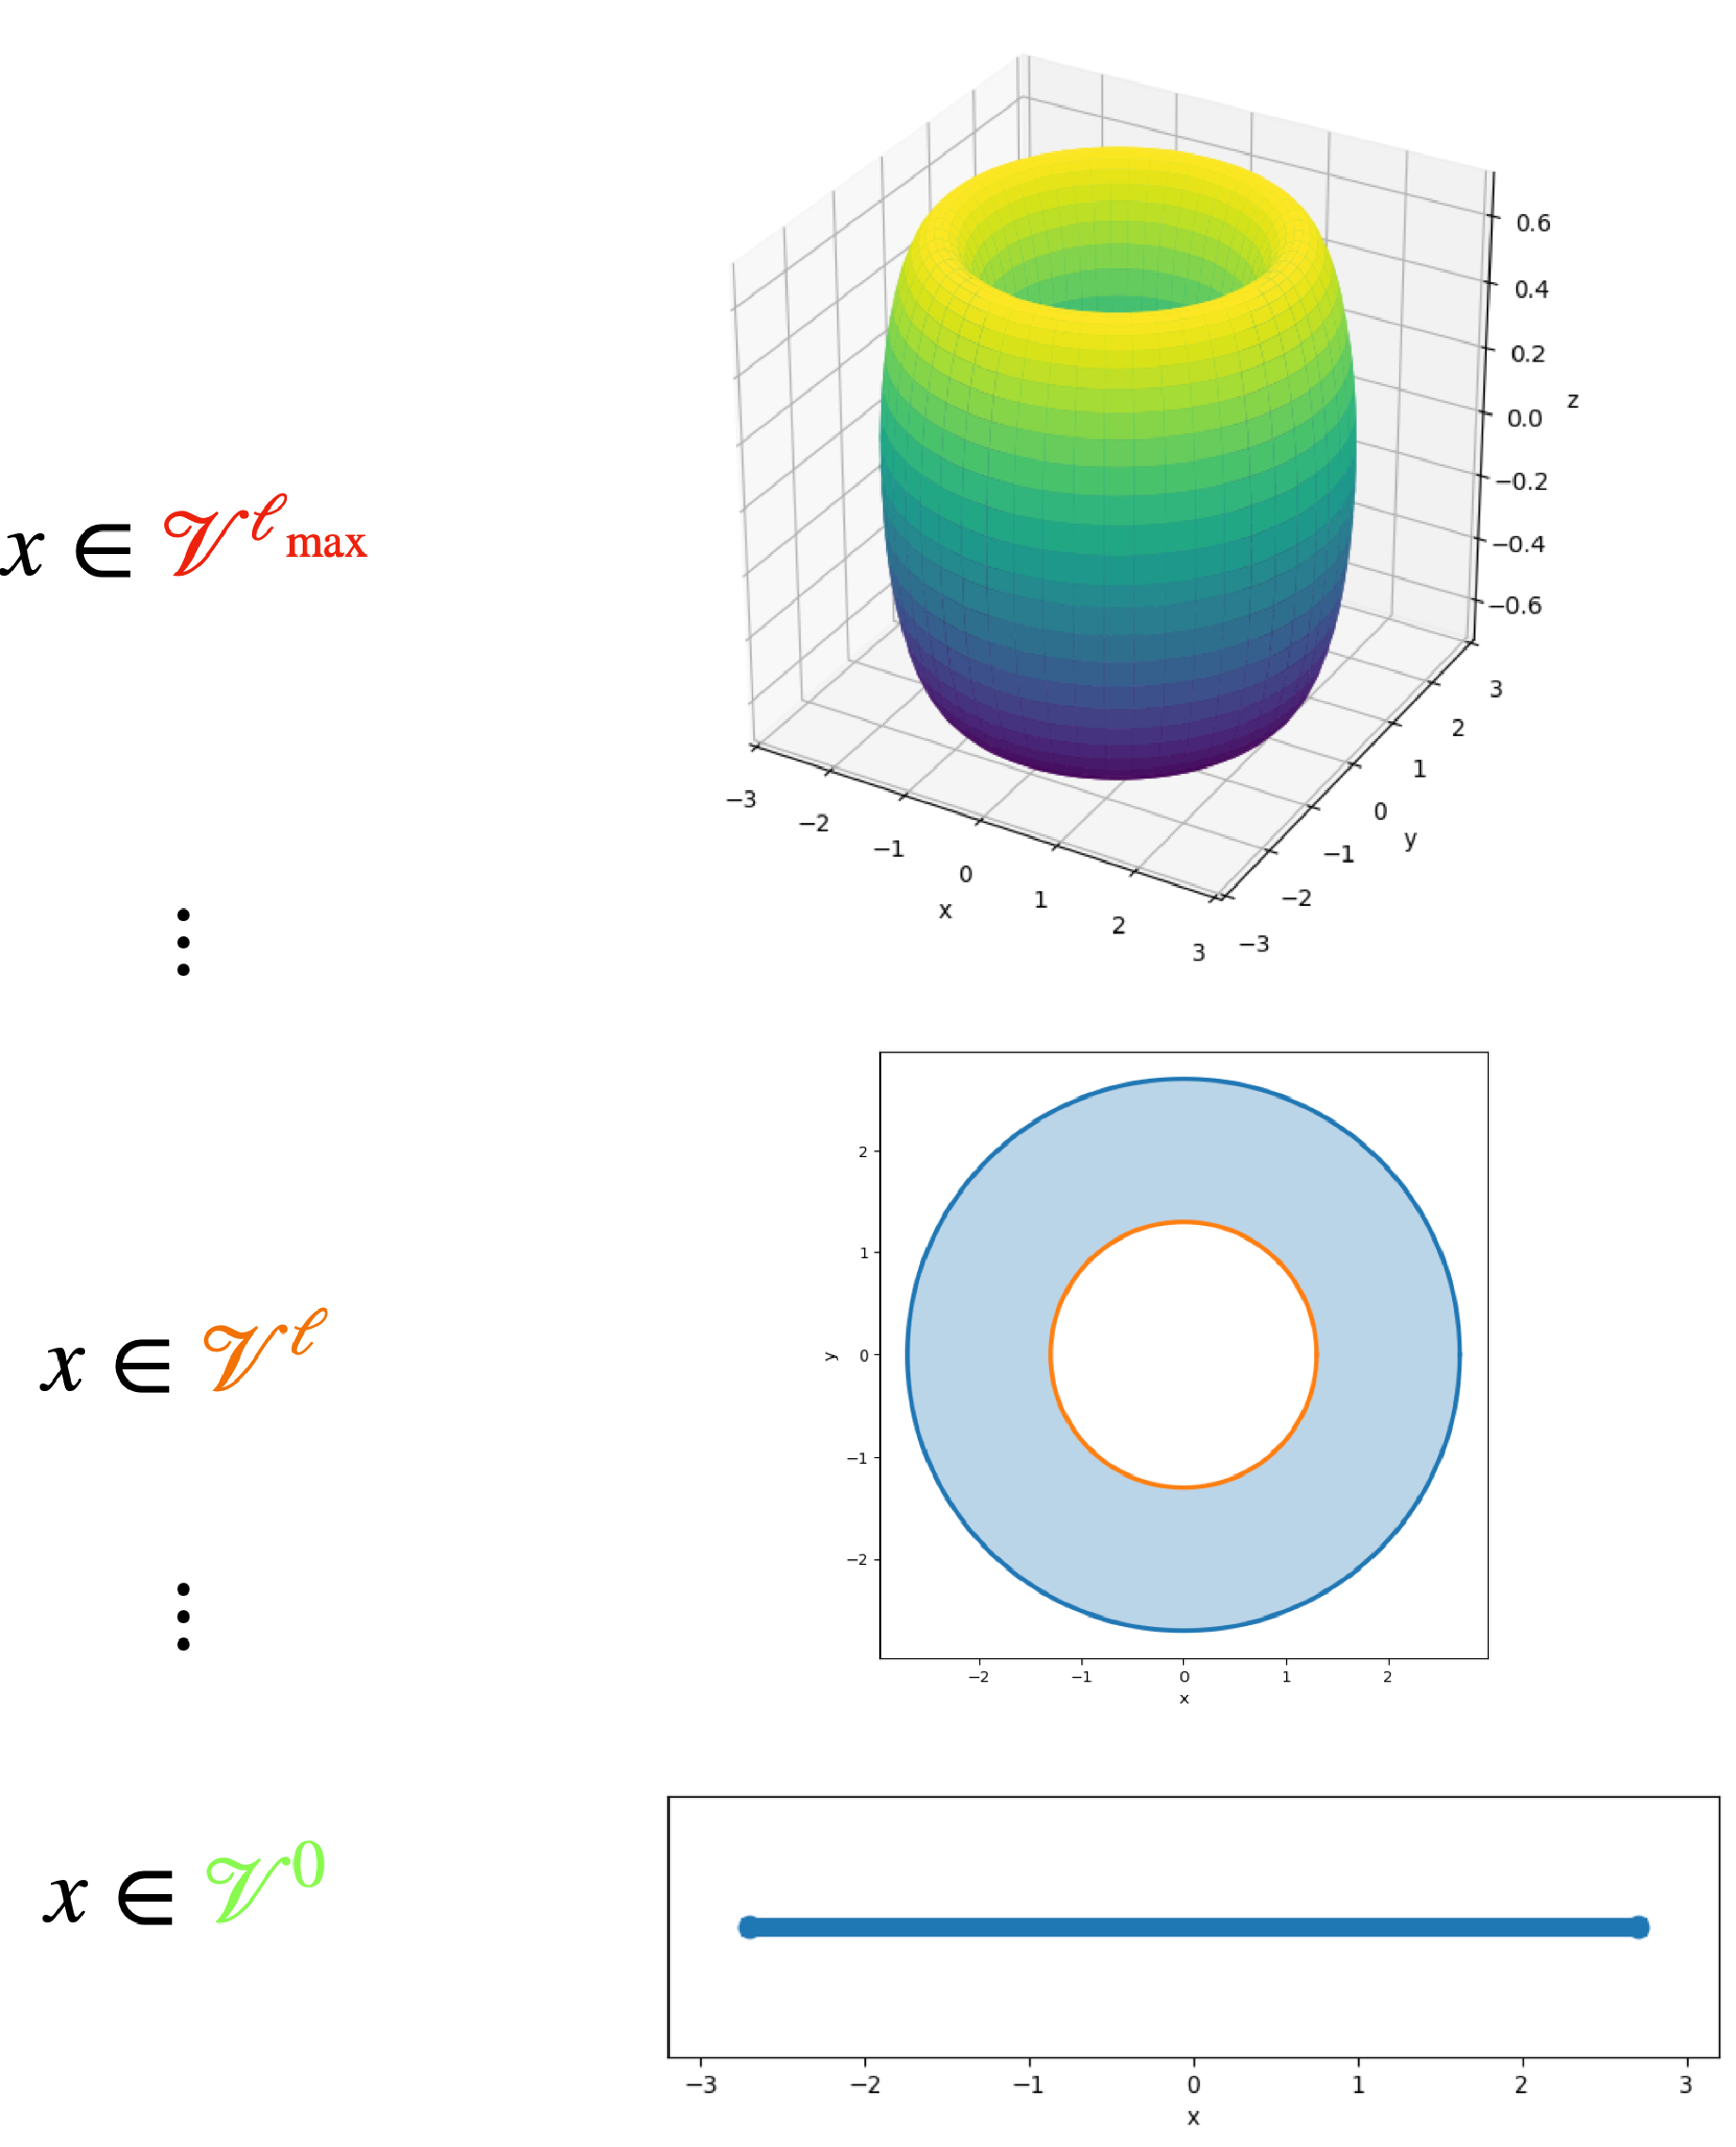
\includegraphics[scale=0.1]{figures/hierarchy_variable2}

\vspace{0.2cm}

\end{minipage}%
}

\end{column}

%---------------------------------
\begin{column}{0.5\textwidth}

\fbox{%
\begin{minipage}{\linewidth}
\centering

%\vspace{0.2cm}

$$
f:\mathcal{X}\rightarrow \boxed{\mathcal{Y}}
$$

Hierarchy in the function space:

${\color{green}\epsilon^0}
\geq\dots\geq
{\color{orange}\epsilon^\ell}
\geq\dots\geq
{\color{red}\epsilon^{\ell_{\max}}}$

\vspace{0.3cm}

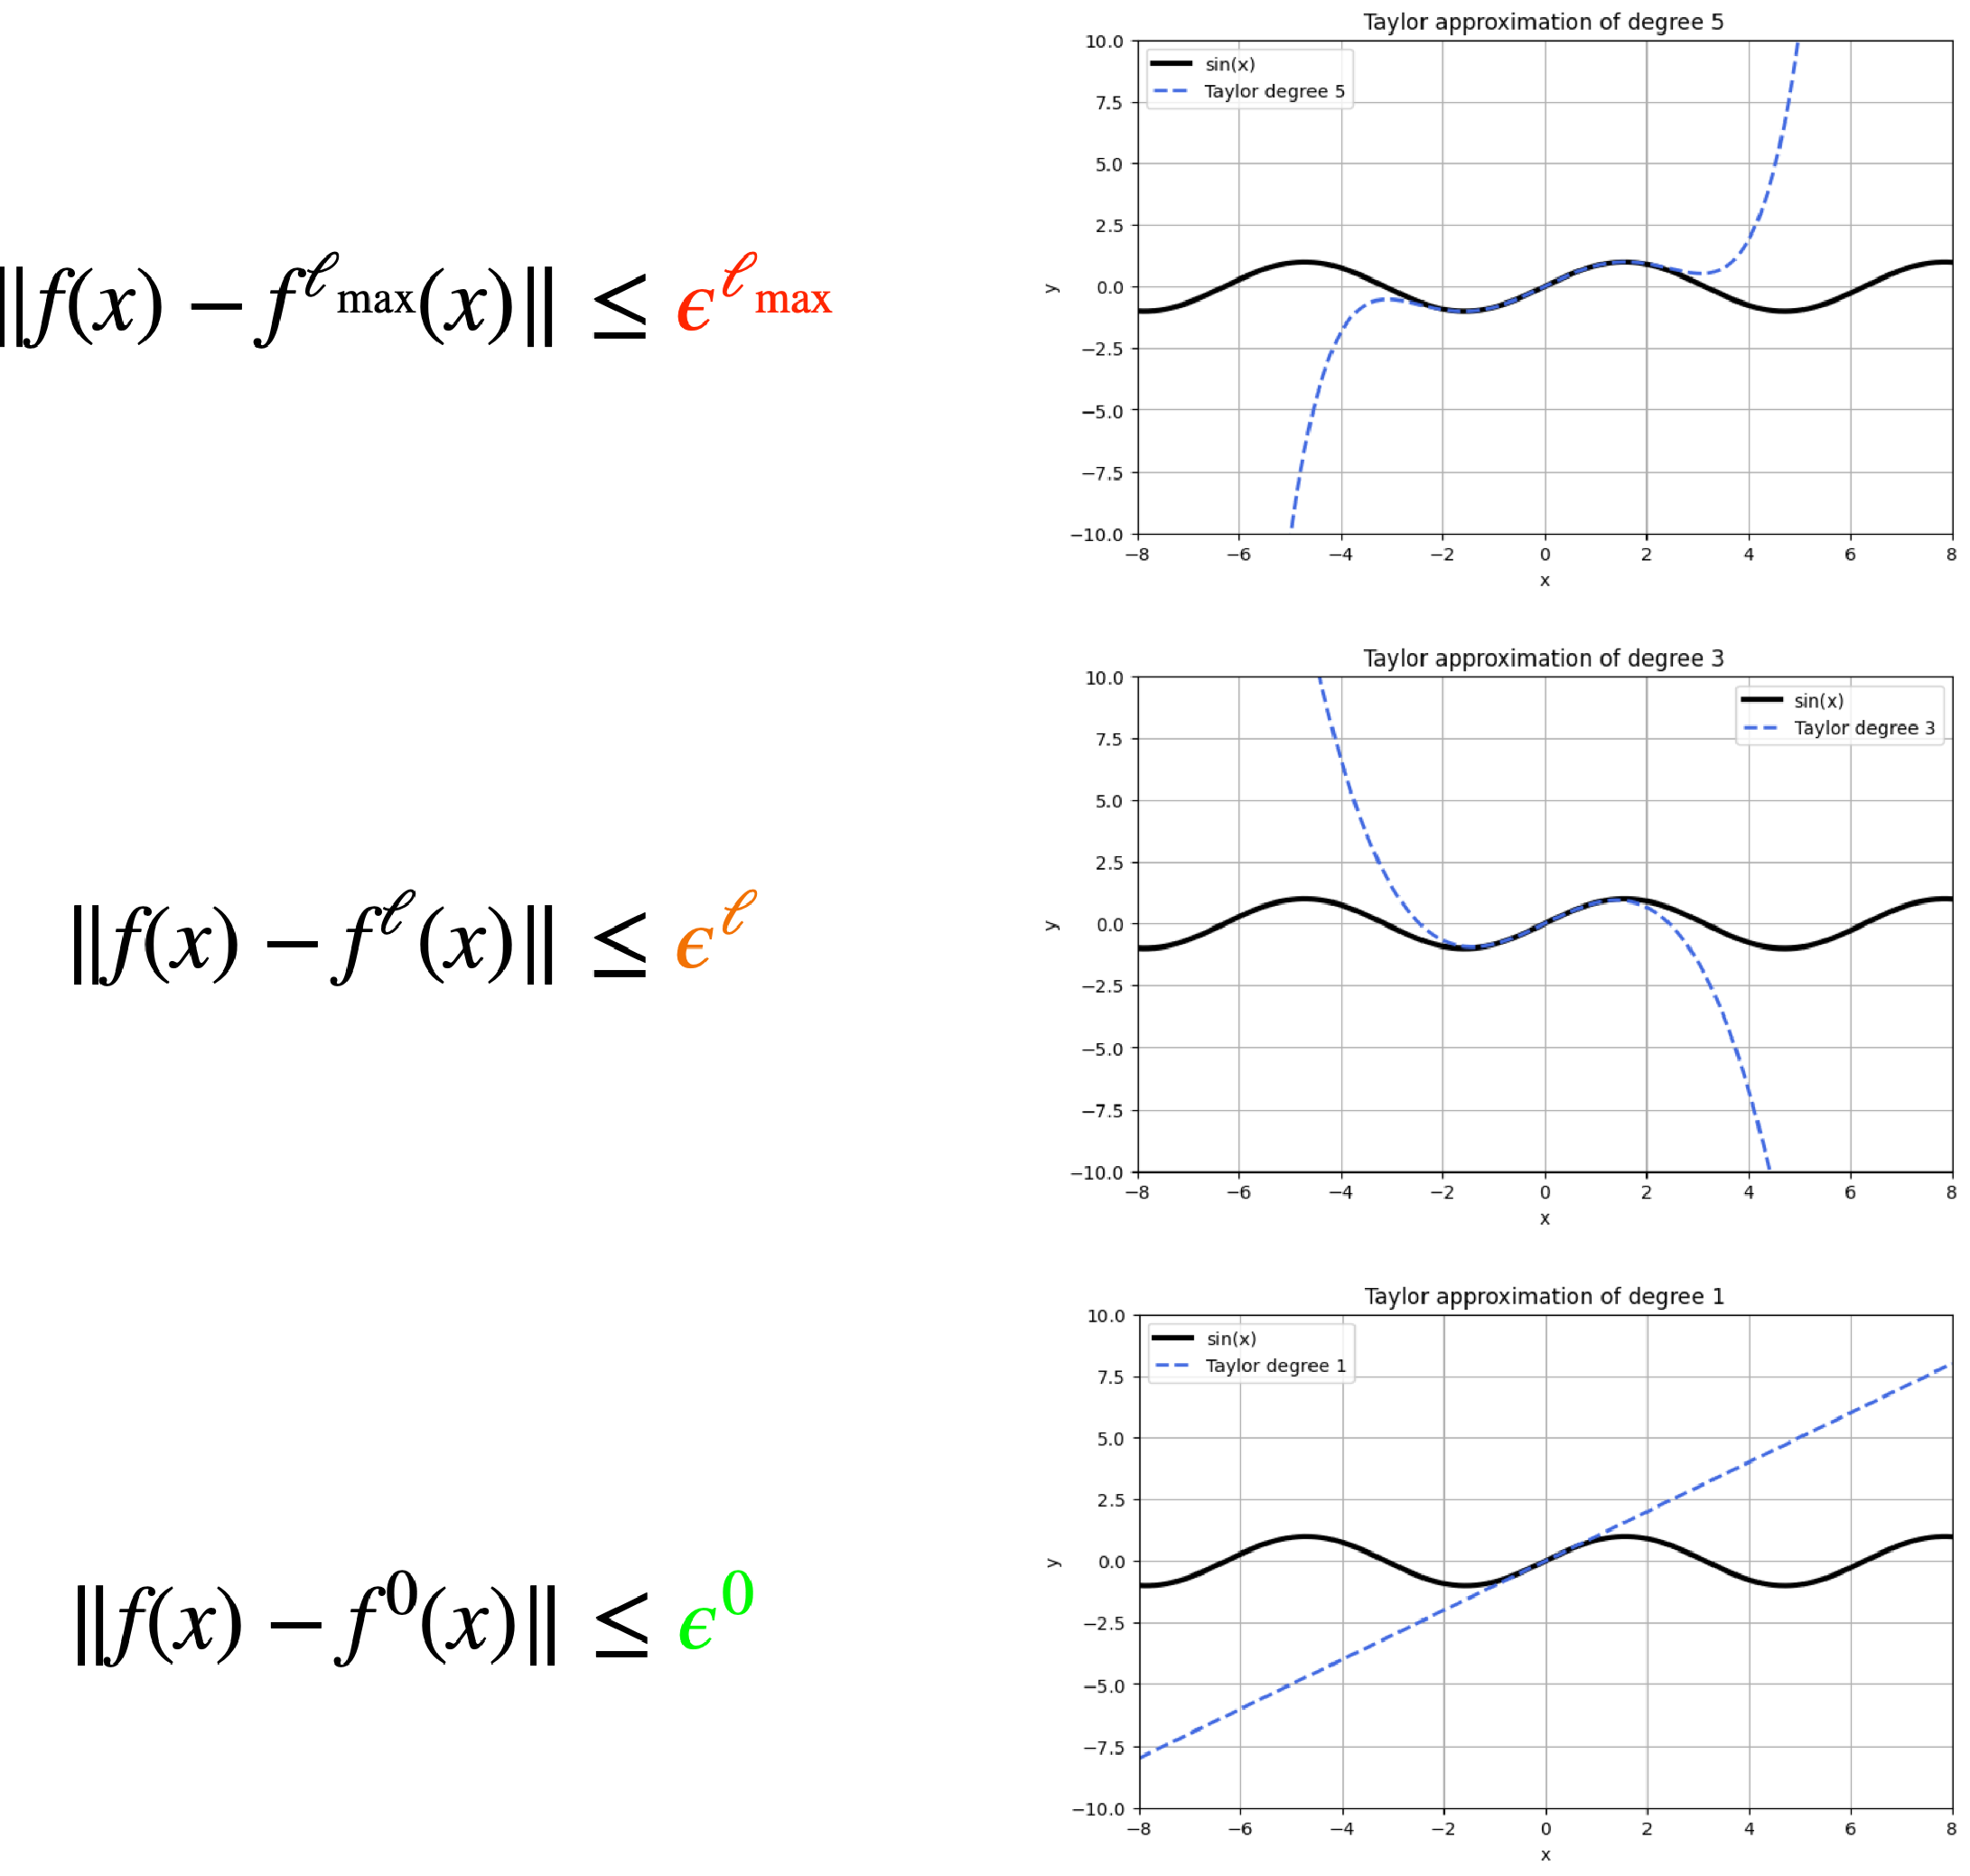
\includegraphics[scale=0.11]{figures/hierarchy_f3}

\vspace{0.2cm}

\end{minipage}%
}

\end{column}

%---------------------------------
\end{columns}
 \end{frame}
 \end{comment}
% \begin{frame}{Can we leverage the multilevel framework? }
 %$$
%\min_x f(x), f:\mathcal{X}\rightarrow \boxed{\mathcal{Y}}
%$$
 %Hierarchy in  the function space: ${\color{green}\epsilon^0}\geq\dots\geq{\color{orange}\epsilon^\ell}\geq \dots\geq{\color{red}\epsilon^{\ell_{\max}}}$
  %\centering
%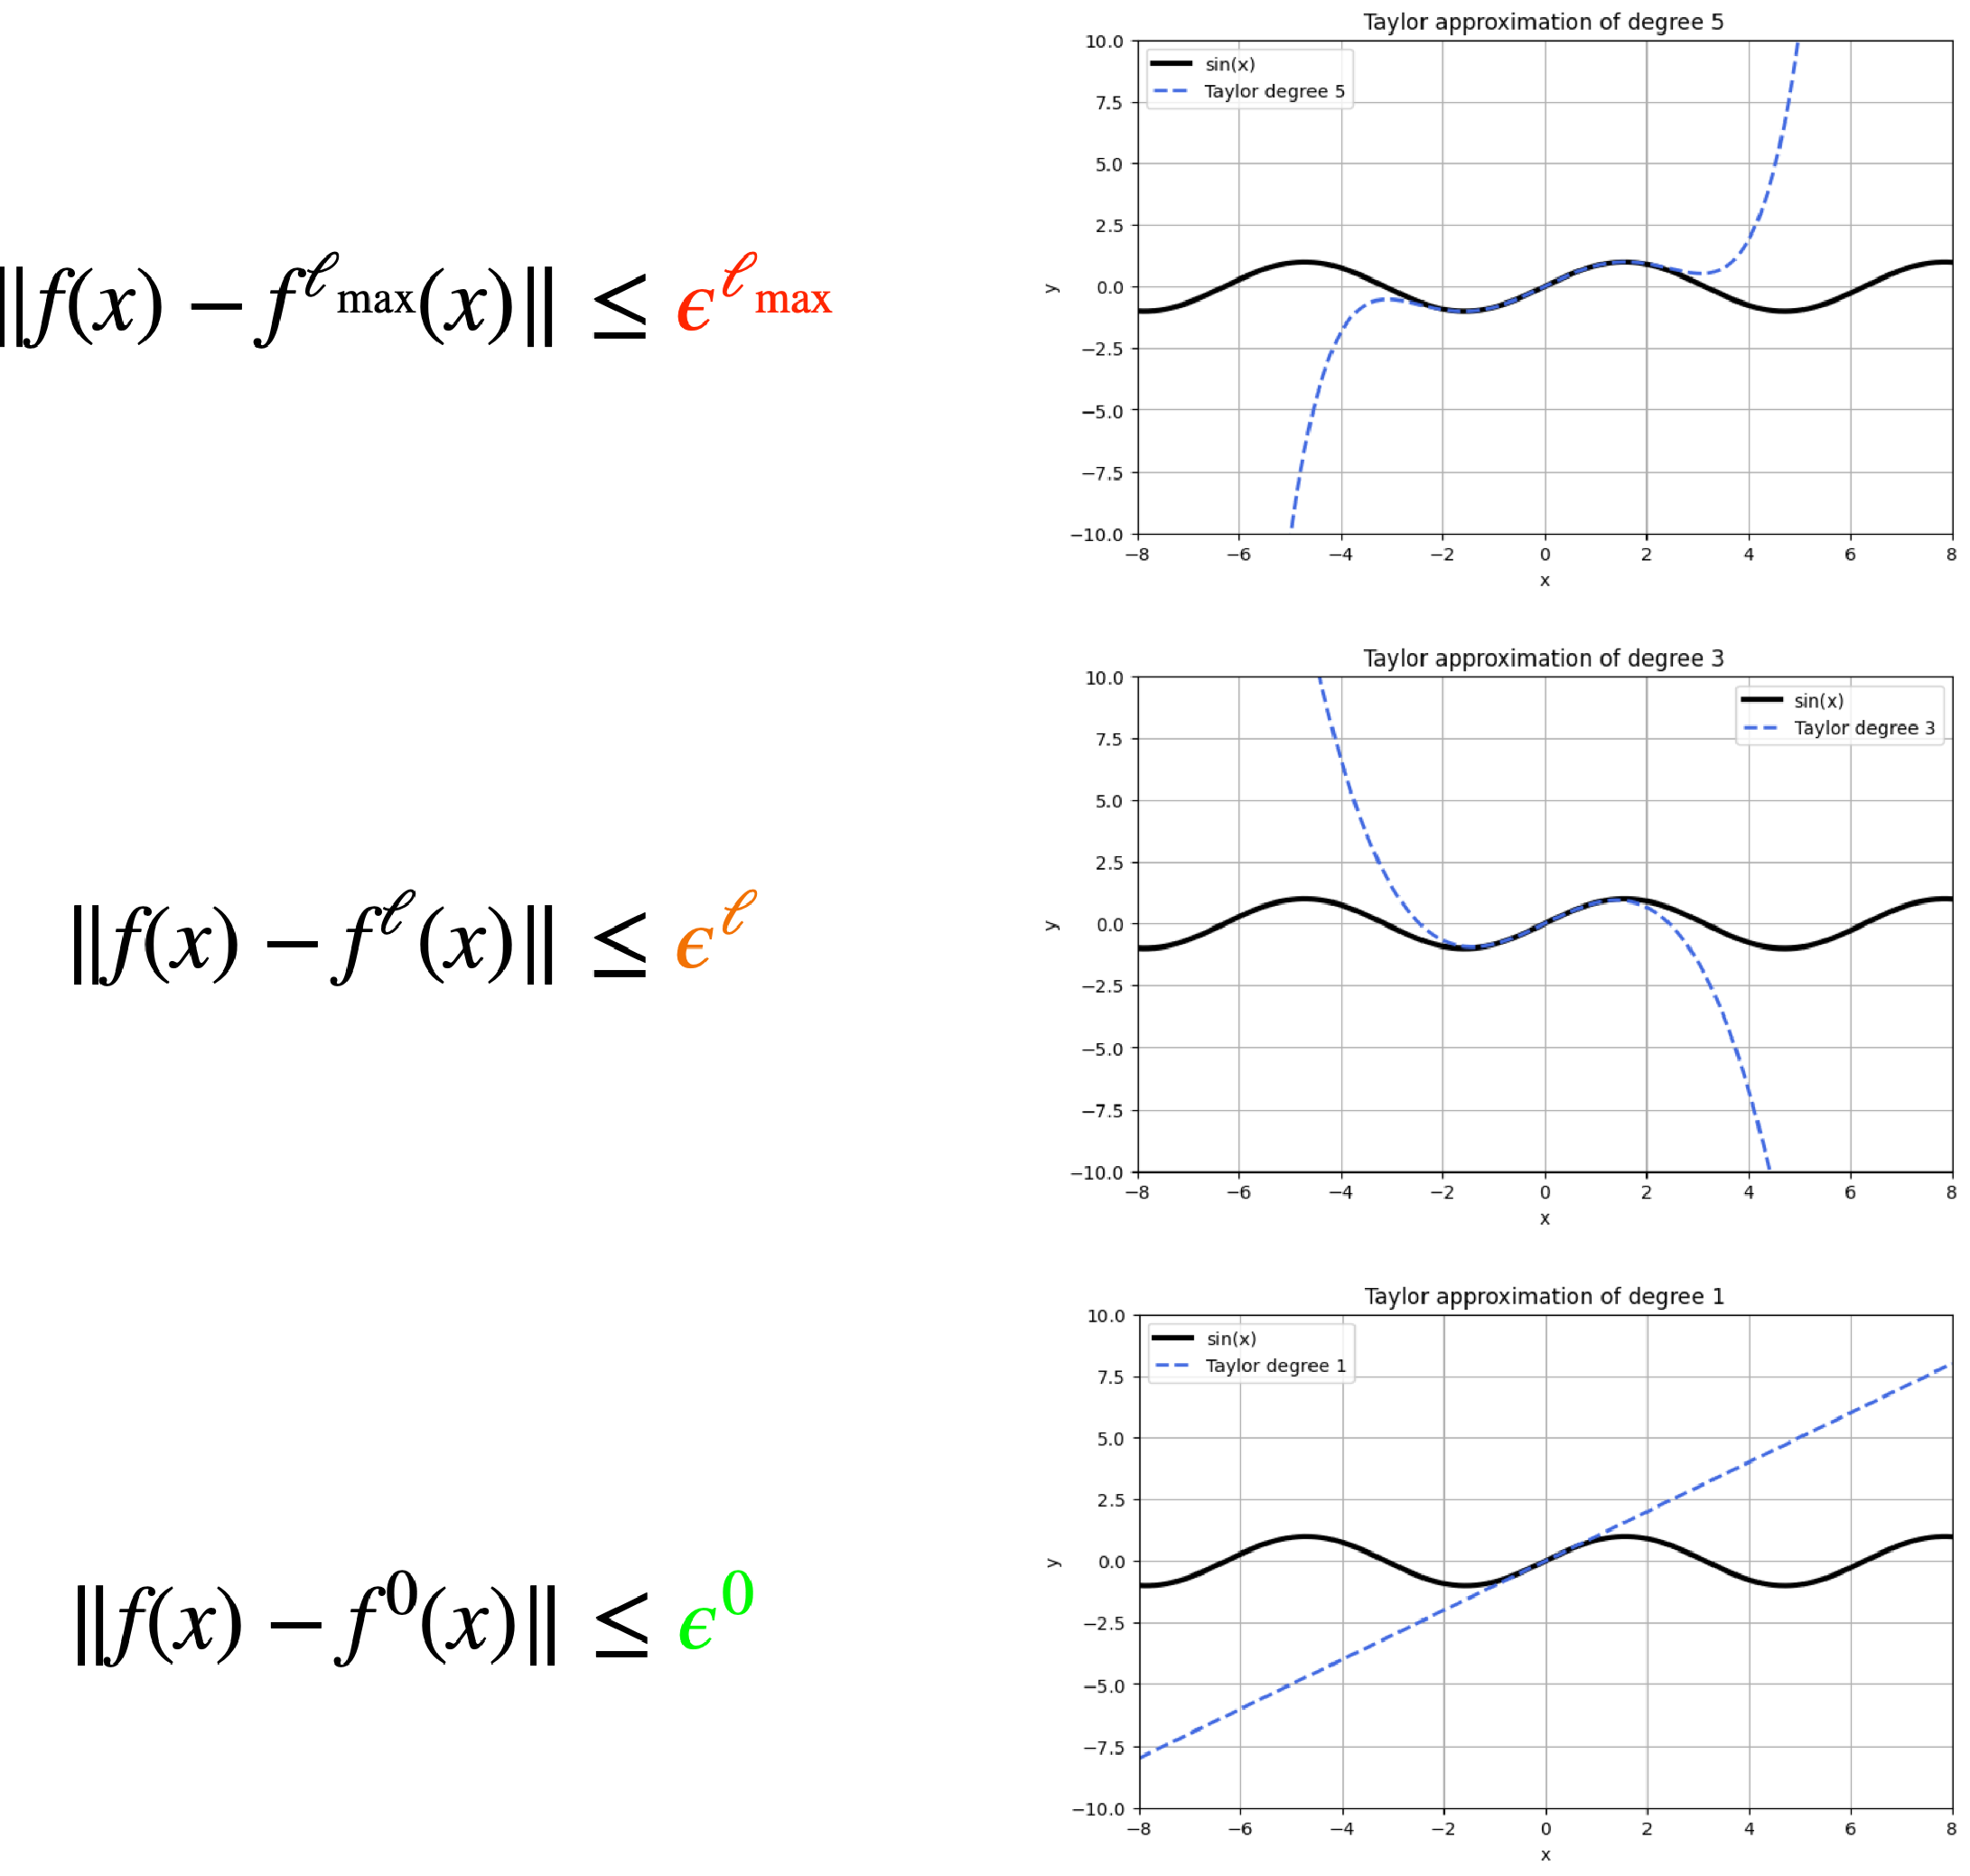
\includegraphics[scale=0.2]{figures/hierarchy_f3}
 %\end{frame}
 
 

 \begin{frame}{Stochastic multilevel iterations}

 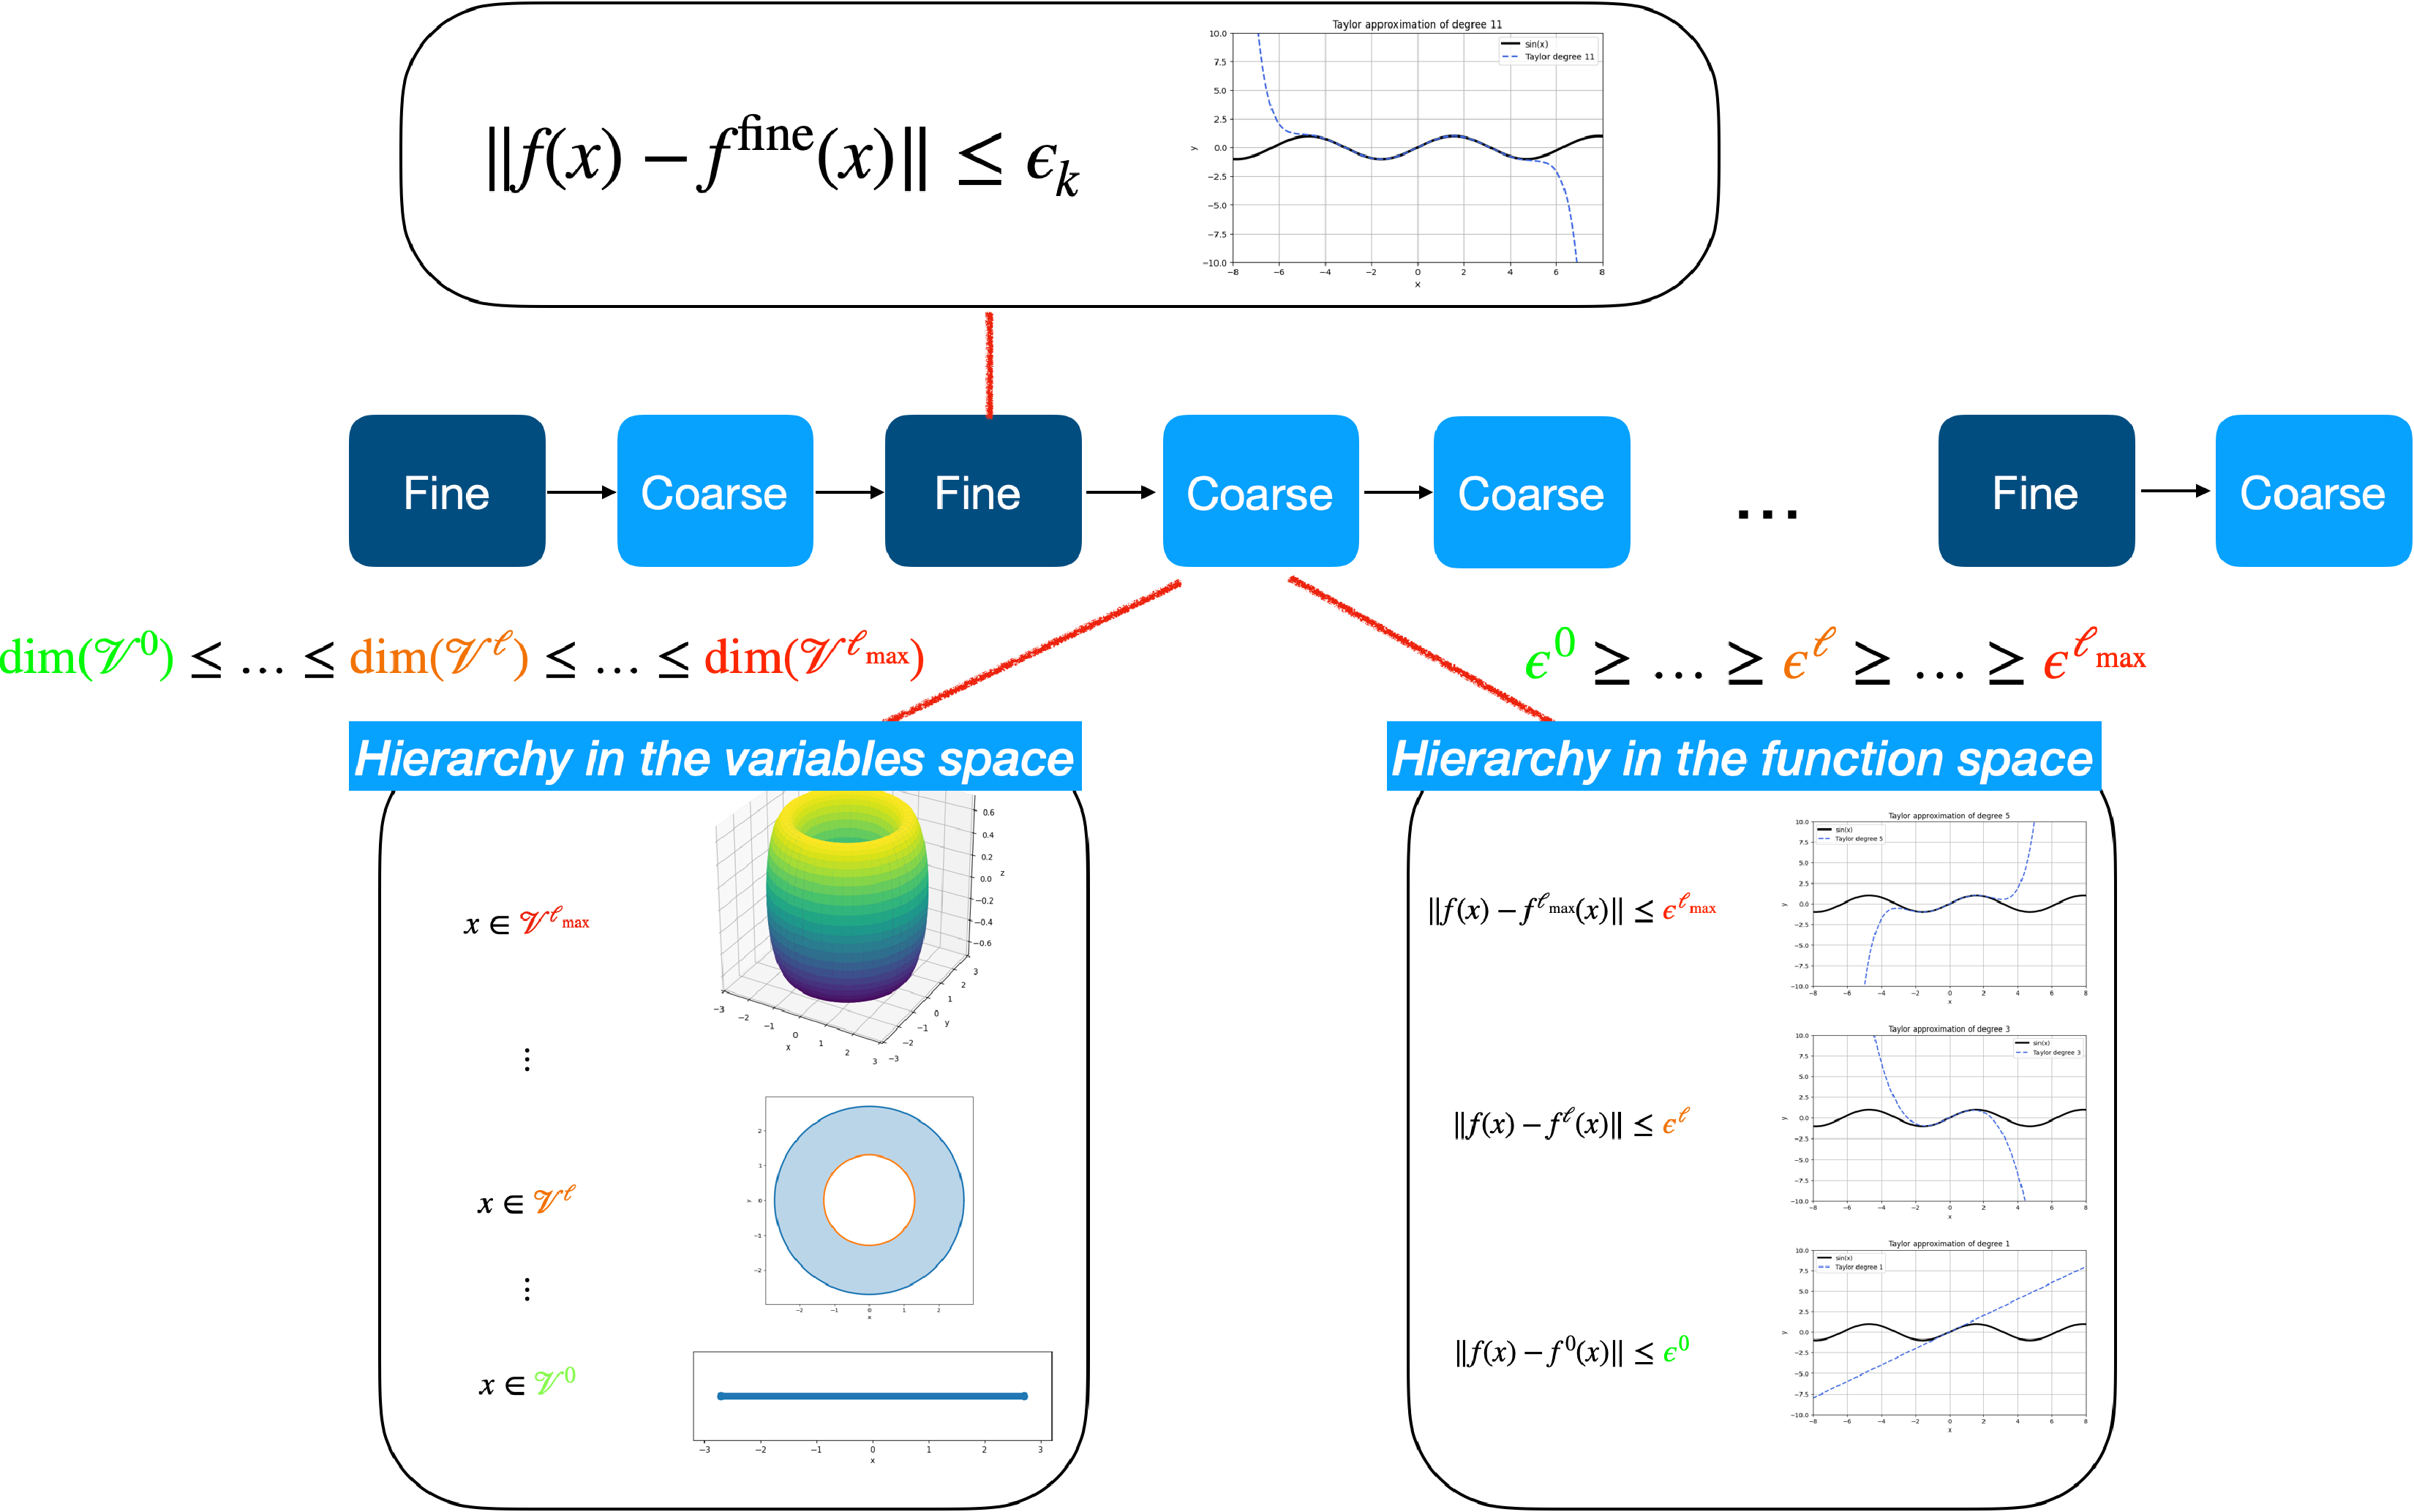
\includegraphics[scale=0.21]{figures/schema_new}

 \end{frame}

 \begin{frame}{Example - Expected risk minimization }
 
 \begin{itemize}
 \item
 Fine level: $$
\tilde f_k(x)=\frac{1}{|\mathcal{S}_k|}\sum_{i\in \mathcal{S}_k}f^{(i)}(x) \quad x\in\mathbb{R}^n, \quad \alert{|\mathcal{S}_k|\nearrow}
$$

\item Coarse level:
\begin{columns}

%====================================================
\begin{column}{0.48\textwidth}

\fbox{%
\begin{minipage}[t][0.58\textheight][t]{0.95\linewidth}

\centering

\vspace{0.2cm}

{\bf Hierarchy in the variables space:}

%\vspace{0.2cm}

Randomly draw
\begin{small}
\[
\mathcal{V}^0
\subseteq\dots\subseteq
\mathcal{V}^\ell
\subseteq\dots\subseteq
\mathcal{V}^{\ell_{\max}}
\subseteq\mathbb{R}^n
\]
\end{small}

\vspace{-0.1cm}

\begin{align*}
\phi_k^\ell(\alert{x^\ell})
&=
\frac{1}{|\mathcal{S}_k|}
\sum_{i\in\mathcal{S}_k}
f^{(i)}(\alert{x^\ell})
\\[0.3cm]
\alert{x^\ell} &\alert{\in \mathcal{V}^{\ell}}
\end{align*}

\end{minipage}%
}

\end{column}

%====================================================
\begin{column}{0.48\textwidth}

\fbox{%
\begin{minipage}[t][0.58\textheight][t]{0.95\linewidth}

\centering

\vspace{0.2cm}

{\bf Hierarchy in the function space:}

%\vspace{0.2cm}

Randomly draw
\begin{small}
\[
\mathcal{S}_k^0
\subseteq\dots\subseteq
\mathcal{S}_k^{\ell}
\subseteq\dots\subseteq
\mathcal{S}_k^{\ell_{\max}}
\subseteq\mathcal{S}_k
\]
\end{small}

%\vspace{0.2cm}

\begin{align*}
\phi_k^\ell(x)
&=
\frac{1}{|\alert{\mathcal{S}_k^\ell}|}
\sum_{i\in\alert{\mathcal{S}_k^\ell}}
f^{(i)}(x)
\\[0.3cm]
x &\in \mathbb{R}^n
\end{align*}

\end{minipage}%
}

\end{column}

%====================================================
\end{columns}  
\end{itemize}\end{frame}







	
	
	
		\begin{frame}{Proposed stochastic multilevel method (2 levels)}
	Mu$^\ell$STREG: First order \alert{adaptive regularization method}
	$$m_k(x_k+s)=\varphi_k(s)+\frac{\lambda_k\|g_k\|}{2}\|s\|^2$$
	\begin{itemize}
	\item  Fine level: $$\varphi_k(s)=f_k+g_k^Ts \quad \alert{f_k\approx f(x_k), \; g_k\approx \nabla f(x_k)}$$ 
	\item Coarse level: 
	\begin{subequations}\label{reg_taylor_model}
$$
\varphi_k(s)=  \coarse_k(\alert{R}x_k+s)+\underbrace{(R\gk-\nabla\coarse_k(Rx_k))^Ts}_{\text{first-order \,coherence}}
$$
    \end{subequations}
    \end{itemize}
	\end{frame}
	
	


	\begin{frame}{The theory - what are we interested in? }
	\begin{center}
	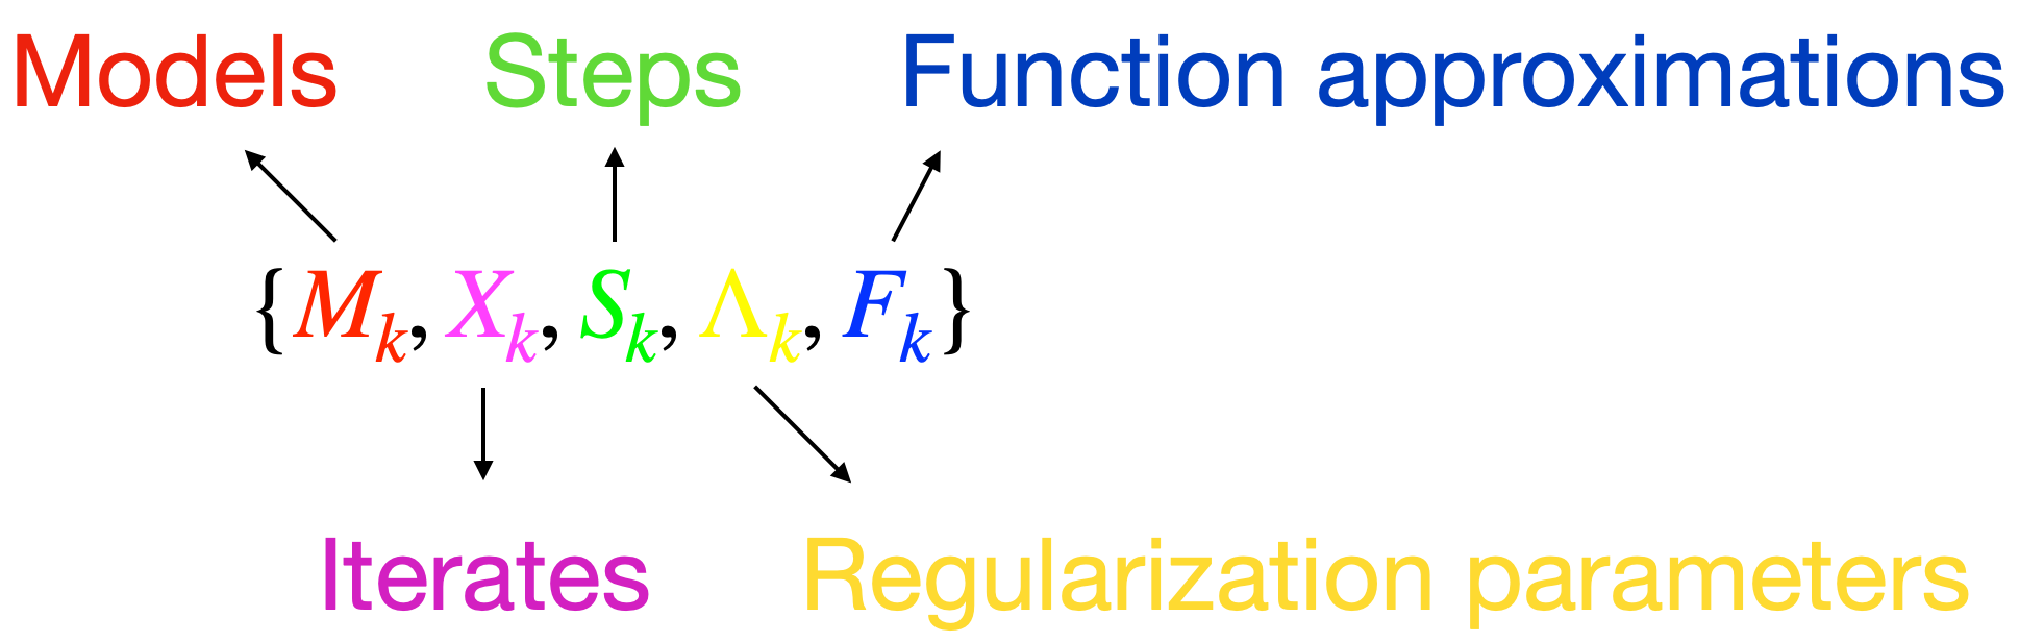
\includegraphics[scale=0.2]{figures/process}
	\end{center}
	\vspace{0.5cm}
	The stochastic process $\{M_k, X_k, S_k, \Lambda_k, F_k\}$, under certain conditions
on the sequences $\{M_k\}$ and $\{F_k\}$
 has desirable convergence
properties with \alert{probability one}. 

	\end{frame}
\begin{frame}{The theory - assumptions [simplified]}



\begin{itemize}
\item 
	 $f:\mathbb{R}^n\rightarrow\mathbb{R}$ and $\coarse_k:\mathbb{R}^{n_c}\rightarrow\mathbb{R}$ with $n\geq n_c$ have Lipschitz continuous gradients 

  %  In the setting of finite sum minimization, cf. Example 1, the assumption is satisfied if all the $f^{(i)}$ are smooth, which is quite a common assumption in this context \cite{garrigos2023handbook}. 
  \item The model $M_k$  to be \alert{$\kappa$-fully linear} around $X_k$ with probability $\alpha$  (\underline{only at fine level!}) 

\item The function approximations $F_k$ to be \alert{sufficiently accurate} ($\epsilon_f$) with probability $\beta$ 
  


\end{itemize}

		\end{frame}
	
	

	
	
		
	

	
\begin{frame}{The theory - results}
  Under suitable choices for           $\epsilon_f$,
     $\alpha$ and $\beta$ can be chosen so that, if the assumptions hold for these values, then the sequence of regularization parameters $\{\Lambda_k\}$ satisfies
     $$
\sum_{k=0}^{\infty}\frac{1}{\Lambda_k^2}<\infty
     $$
     and the sequence of iterates  $\{X_k\}$ satisfy
$$
\lim_{k\rightarrow\infty}\|\nabla_x f(X_k)\|=0
$$
     almost surely.
\end{frame}

\begin{frame}{Numerical results - Finite sum minimization}
\begin{block}{The problem}
\begin{equation*}
    \min_{x \in  \mathbb{R}^n}  F(x) =  \frac{1}{2N}\sum_{i=1}^N (y_i - \frac{1}{1 + \text{exp}(-y_ix^Tz_i)})^2,
\end{equation*}
with $(z_i,y_i)\in \mathbb{R}^n \times \{0,1\}$, for every $i=1,\dots,N$. 
\end{block}
\vspace{0.3cm}
\begin{block}{The methods}
\begin{itemize}
\item MU$^1$STREG: one level ($\approx$ STORM [Chen, et all. 2018])
\item MU$^3$STREG: three levels
\item Adagrad [J. Duchi, E. Hazan, and Y. Singer. (2011)]
\item SVRG [R. Johnson and T. Zhang. (2013)]
\end{itemize}
$$x_{k+1}=x_k-\alpha\left[\frac{1}{b}\sum_{i_k\in I_k}\nabla f^{i_k}(x_k) +\textcolor{blue}{ \left(\nabla f(\tilde{x}_0)-\frac{1}{b}\sum_{i_k\in I_k}\nabla f^{i_k}(\tilde{x}_0)\right)}\right],$$ 
where $\tilde{x}_0$ is updated every $m$ iterations 
\end{block}
	\end{frame}


	\begin{frame}{Results: comparison against  MU$^1$STREG{} and SVRG}
	 \begin{table}[h!]
\centering
\tiny
\begin{tabular}{|lccc|}
\hline
\multicolumn{4}{|c|}{MUSH}\\  
\hline
 & \multicolumn{1}{|c|}{SVRG }                   & \multicolumn{1}{c|}{MU$^1$STREG} & MU$^3$STREG \\\hline
\rowcolor{yellow}
\multicolumn{1}{|l|}{\textbf{Avg. \%tA}}               & \multicolumn{1}{c|}{98.69}                                                   & \multicolumn{1}{c|}{97.68}                                                    & 97.74                                                    \\
\multicolumn{1}{|l|}{\textbf{StD \%tA}}                & \multicolumn{1}{c|}{0.25}                                                         & \multicolumn{1}{c|}{0.50}                                                     & 0.48                                                     \\
\rowcolor{lightgray}
\multicolumn{1}{|l|}{\textbf{Avg. \#f/g}}              & \multicolumn{1}{c|}{341.89}                                                         & \multicolumn{1}{c|}{216.78}                                                   & 35.48                                                    \\

\multicolumn{1}{|l|}{\textbf{StD \#f/g}}               & \multicolumn{1}{c|}{722.65}                                                  & \multicolumn{1}{c|}{30.69}                                                    & 9.95                                                     \\ \hline
\multicolumn{4}{|c|}{A9A}                                                                                                                                                                                                                                                                                     \\ \hline
 & \multicolumn{1}{|c|}{SVRG }                   & \multicolumn{1}{c|}{MU$^1$STREG} & MU$^3$STREG \\\hline
\rowcolor{yellow}
\multicolumn{1}{|l|}{\textbf{Avg. \%tA}}               & \multicolumn{1}{c|}{85.00}                                                       & \multicolumn{1}{c|}{84.65}                                                    & 84.83                                                    \\
\multicolumn{1}{|l|}{\textbf{StD \%tA}}                & \multicolumn{1}{c|}{0.05}                                                          & \multicolumn{1}{c|}{0.04}                                                     & 0.07                                                     \\
\rowcolor{lightgray}
\multicolumn{1}{|l|}{\textbf{Avg. \#f/g}}              & \multicolumn{1}{c|}{840.77}                                                & \multicolumn{1}{c|}{207.68}                                                   & 90.87                                                    \\
\multicolumn{1}{|l|}{\textbf{StD \#f/g}}               & \multicolumn{1}{c|}{300.51}                                                    & \multicolumn{1}{c|}{53.97}                                                    & 30.31                                                    \\ \hline
\multicolumn{4}{|c|}{IJCNN1}                                                                                                                                                                                                                                                                                  \\ \hline
& \multicolumn{1}{|c|}{SVRG }                   & \multicolumn{1}{c|}{MU$^1$STREG} & MU$^3$STREG \\\hline
\rowcolor{yellow}
\multicolumn{1}{|l|}{\textbf{Avg. \%tA}}               & \multicolumn{1}{c|}{91.68}                                                       & \multicolumn{1}{c|}{91.10}                                                    & 91.13                                                    \\
\multicolumn{1}{|l|}{\textbf{StD \%tA}}                & \multicolumn{1}{c|}{0.00}                                                           & \multicolumn{1}{c|}{0.25}                                                     & 0.09                                                     \\
\rowcolor{lightgray}
\multicolumn{1}{|l|}{\textbf{Avg. \#f/g}}              & \multicolumn{1}{c|}{553.87}                                                       & \multicolumn{1}{c|}{6.20}                                                     & 7.09                                                     \\

\multicolumn{1}{|l|}{\textbf{StD \#f/g}}               & \multicolumn{1}{c|}{1.64}                                                              & \multicolumn{1}{c|}{0.97}                                                     & 0.64                                                     \\ \hline
\multicolumn{4}{|c|}{MNIST}                                                                                                                                                                                                                                                                                   \\ \hline
 & \multicolumn{1}{|c|}{SVRG }                   & \multicolumn{1}{c|}{MU$^1$STREG} & MU$^3$STREG \\\hline
\rowcolor{yellow}
\multicolumn{1}{|l|}{\textbf{Avg. \%tA}}               & \multicolumn{1}{c|}{90.43}                                               & \multicolumn{1}{c|}{89.80}                                                    & 89.82                                                    \\
\multicolumn{1}{|l|}{\textbf{StD \%tA}}                & \multicolumn{1}{c|}{0.13}                                                     & \multicolumn{1}{c|}{0.04}                                                     & 0.05                                                     \\
\rowcolor{lightgray}
\multicolumn{1}{|l|}{\textbf{Avg. \#f/g}}              & \multicolumn{1}{c|}{17843.40}                                                     & \multicolumn{1}{c|}{2923.02}                                                  & 414.15                                                   \\
\multicolumn{1}{|l|}{\textbf{StD \#f/g}}               & \multicolumn{1}{c|}{6336.56}                                                  & \multicolumn{1}{c|}{497.15}                                                   & 16.37   \\ \hline                                                
\end{tabular}
\caption{Comparison between MU$^1$STREG{}, MU$^3$STREG{} and SVRG. Average of maximum classification accuracy reached and number of evaluations, with corresponding standard deviation. }
\end{table}

\end{frame}


\begin{frame}{Results: comparison against  MU$^1$STREG{} and Adagrad}

\begin{figure}[h!]
    \centering
    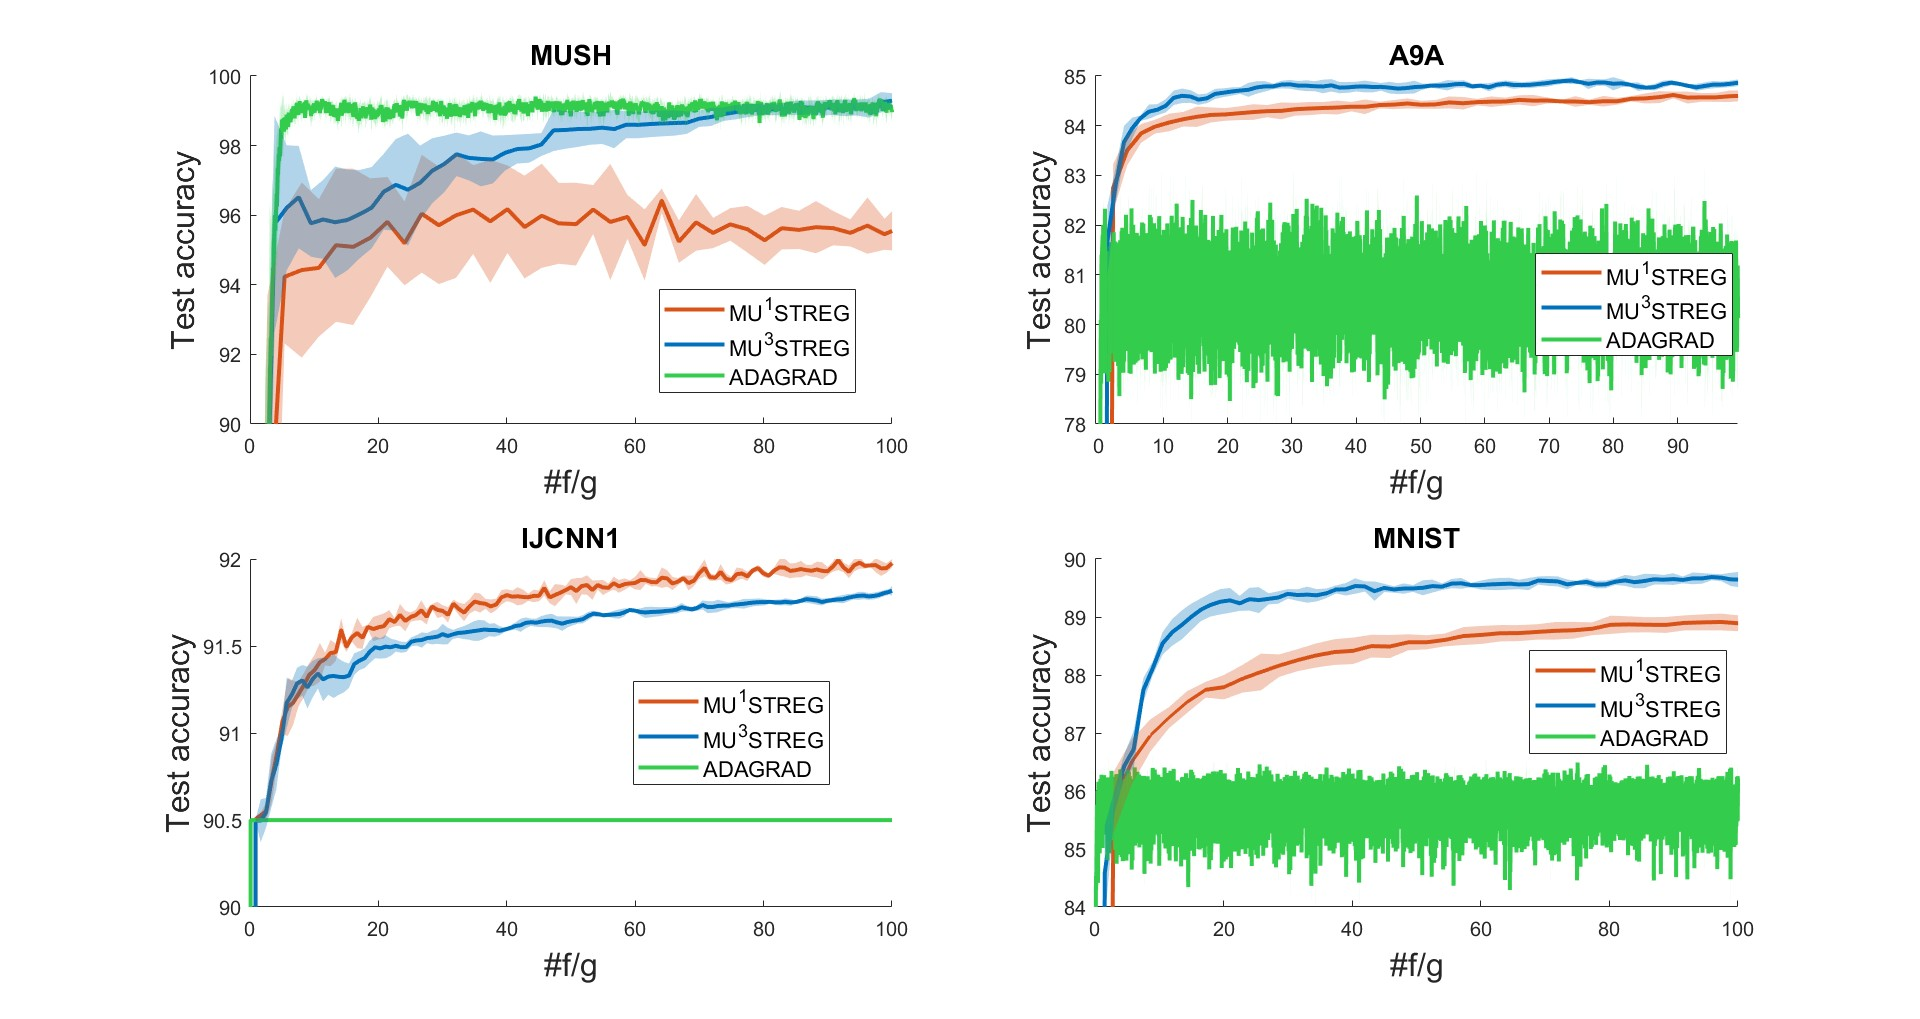
\includegraphics[width=\linewidth]{figures/LEAST-SQUARES_acc_vs_ev_SHADED.jpg}
    \caption{ Classification accuracy on the testing set along the number of  weighted evaluations of gradients and functions.}
    \label{fig: acc vs. ev.}
\end{figure}
	
	\end{frame}
	

		
		
\begin{frame}{Conclusions}
Multilevel framework:
\begin{itemize}
\item Flexible framework to accelerate large scale problems, adaptable to different contexts
\end{itemize}
MU$^\ell$STREG
\begin{itemize}
\item allows for hierarchies in the both variable and function spaces;
\vskip 3pt
\item is the first stochastic framework for multilevel methods;
\vskip 3pt
\item Applied to \alert{finite sum problems}:  outperforms tested methods; 
wrt to the classical deterministic ML framework: \structure{it does not need the evaluation of the function/gradient over the full samples set along all the iterations}.
\end{itemize}

\begin{block}{}
 \begin{small} \structure{F. Marini, M. Porcelli,  E. Riccietti, 
   \textbf{A multilevel stochastic regularized first-order method with application to finite sum minimization}, 2024, \textit{arXiv:2412.11630}, accepted in Mathematics of computation}  
\end{small}
\end{block}

         
\end{frame}

\begin{frame}{STOP workshop}
\begin{center}
\includegraphics[scale=0.3]{../../loghi_firme/ENS_foto.jpeg}\\
STructured OPtimization for inverse and learning problems\\
28 september - 01 october 2026\\
ENS Lyon
\url{https://perso.ens-lyon.fr/elisa.riccietti/STOP.php}
\end{center}
\vspace{0.5cm}
 \pause\begin{center}
    \alert{\Large{ \textit{Thank you for your attention!}}}
\end{center} 
\end{frame}

\appendix
\begin{frame}{Numerical results - Finite sum minimization}

\begin{figure}[h!]
    \centering
    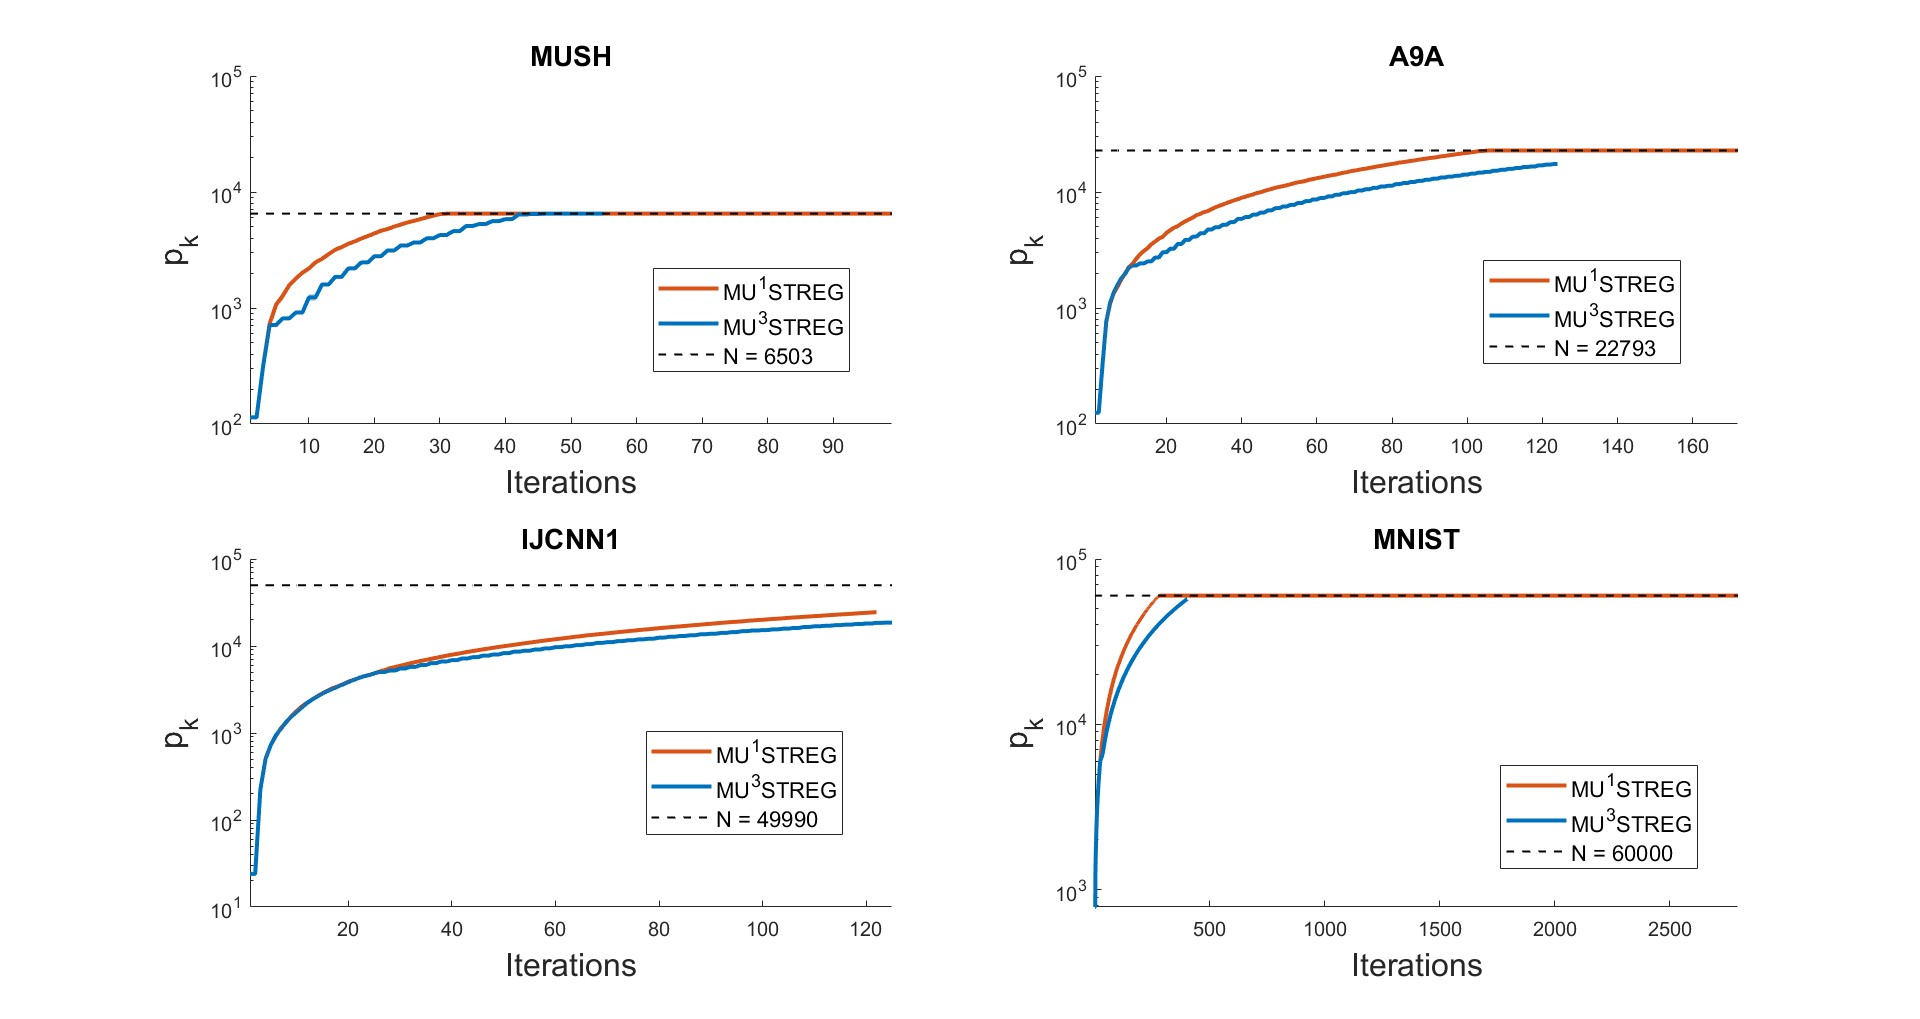
\includegraphics[width=\linewidth]{figures/LEAST-SQUARES_p_k_vs_ev_SHADED.jpg}
    \caption{Cardinality of the sample set at the finest level and the full size $N$ along the iterations. $\lvert\mathcal{S}_k^{\ell_{\max}}\rvert=p_k:=\min\{N,\max\{100k+n+2, \alert{\lambda_k^2\}}\}$ }
    \label{fig: pk vs. ev.}
\end{figure}
	\end{frame}


%\begin{frame}{SVRG update}
%$$x_{k+1}=x_k-\alert{\alpha}\quadre{\frac{1}{b}\sum_{i_k\in I_k}\nabla f^{i_k}(x_k) +\textcolor{blue}{ \tonde{\nabla f(\tilde{x}_0)-\frac{1}{b}\sum_{i_k\in I_k}\nabla f^{i_k}(\tilde{x}_0)}}},$$ 
%where $\tilde{x}_0$ is updated every $m$ iterations, when the full gradient is re-evaluated. 
%\end{frame}

\begin{frame}{The theory - assumptions}
Let $\mathcal{F}^{M\, F}_{k-1/2}$ be
 the $\sigma$-algebra generated by $M_0,\dots,M_{k}$
and $F_0,\dots,F_{k-1}$ and  $\mathcal{F}^{M\, F}_{k-1}$ be
 the $\sigma$-algebra generated by $M_0,\dots,M_{k-1}$
and $F_0,\dots,F_{k-1}$.


\begin{itemize}
\item 
	 $f:\mathbb{R}^n\rightarrow\mathbb{R}$ and $\coarse_k:\mathbb{R}^{n_c}\rightarrow\mathbb{R}$ with $n\geq n_c$ have Lipschitz continuous gradients 

  %  In the setting of finite sum minimization, cf. Example 1, the assumption is satisfied if all the $f^{(i)}$ are smooth, which is quite a common assumption in this context \cite{garrigos2023handbook}. 
  \item $M_k$ \alert{$\alpha$-probabilistically $\kappa$-fully linear models}: $
\mathbb{P}(I_k|\mathcal{F}^{M\, F}_{k-1}) \geq \alpha,
$ $
I_k = \{M_k \text{ is a } \kappa\text{ -fully linear model of } f \text{ around } X_k\} 
$
\item $F_k$ \alert{$\beta$-probabilistically $\epsilon_f$-accurate estimates}: $\mathbb{P}(J_k|\mathcal{F}^{M\, F}_{k-1/2}) \geq \beta$, 
$
J_k = \{F_k,F_k^s \text{ are } \epsilon_f\text{-accurate estimates of } f(x_k) \text{ and } f(x_k+s_k), \text{ respectively, around } X_k\} 
$ $$
  \lvert f_k-f(x_k)\rvert\leq \frac{\epsilon_f}{\lambda_k^2} \text{ and } \lvert f_k^s-f(x_k+s_k)\rvert\leq \frac{\epsilon_f}{\lambda_k^2}.
  $$
  


\end{itemize}

		\end{frame}


\begin{frame}{Convergence theory: definitions}
\begin{block}{Definition 1}
Suppose that $\nabla f$ is Lipschitz continuous. Given $\lambda_k>0$, a function $m$ is a \textcolor{red}{$\kappa$-fully linear model} of $f$ around the iterate $x_k$ provided for $\kappa = (\kappa_f , \kappa_g)$, that for all $y$ in a neighborhood of $x_k$:
\begin{align*}
\|\nabla_x f (y) - \nabla_x m(y)\|\leq \frac{\kappa_g}{\lambda_k}, \\
|f (y) - m(y)| \leq \frac{\kappa_f}{\lambda_k^2}.
\end{align*}    
\end{block}   
\begin{block}{Definition 2}
A sequence of random models $\{M_k\}$ is said to be \textcolor{red}{$\alpha$-probabilistically $\kappa$-fully linear} with respect to the corresponding sequence $\{X_k,\Lambda_k\}$ 
if the events
$$
I_k = \{M_k \text{ is a } \kappa\text{ -fully linear model of } f \text{ around } X_k\} 
$$
satisfy the condition
$$
\mathbb{P}(I_k|\mathcal{F}^{M\cdot F}_{k-1}) \geq \alpha.
$$
where $\mathcal{F}^{M\, F}_{k-1}$
is the $\sigma$-algebra generated by $M_0,\dots,M_{k-1}$
and $F_0,\dots,F_{k-1}$
\end{block}
\end{frame}
\begin{frame}{Convergence theory: definitions}
\begin{block}{Definition 3}
The estimates $f_k$ and $f_k^s$ are said to be \textcolor{red}{$\epsilon_f$-accurate} estimates of $f(x_k)$ and $f(x_k+s_k)$ respectively, for a given $\lambda_k$ if 
  $$
  \lvert f_k-f(x_k)\rvert\leq \frac{\epsilon_f}{\lambda_k^2} \text{ and } \lvert f_k^s-f(x_k+s_k)\rvert\leq \frac{\epsilon_f}{\lambda_k^2}.
  $$
    
\end{block}
\begin{block}{Definition 4}
A sequence of random estimates $\{F_k,F_k^s\}$ is said to be \textcolor{red}{$\beta$-probabilistically $\epsilon_f$-accurate} with respect to the corresponding sequence $\{X_k,\Lambda_k,S_k\}$
if the events
\begin{align*}
J_k =& \{F_k,F_k^s \text{ are } \epsilon_f\text{-accurate estimates of } f(x_k) \\
& \text{ and } f(x_k+s_k), \text{ respectively, around } X_k\}
\end{align*}
 

satisfy the condition
$$
\mathbb{P}(J_k|\mathcal{F}^{M\cdot F}_{k-1/2}) \geq \beta,
$$
where $\epsilon_f$ is a fixed constant.    
\end{block}
    
\end{frame}




\begin{frame}{Data sets}
    The data sets are divided into a training set and a testing set as specified in Table below.
\begin{table}[h!]
    \centering
    \begin{tabular}{llll}
    Data set        & nr. of features ($n$)   & Training set size ($N$)& Testing set size ($N_t$) \\ \hline
    MNIST  & 784                     & 60000                  & 10000 \\
MUSH  & 112                     & 6503                   & 1621\\
    A9A    & 123                     & 22793                  & 9768\\
    IJCNN1 & 22                      & 49990                  & 91701\\
    \end{tabular}
    \caption{Data sets with number of features $n$ and number of instances of the training set $N$ and the testing set $N_t$.}
    \label{tab: datasets}
\end{table}
\end{frame}



			
\end{document}